\documentclass{article}

% if you need to pass options to natbib, use, e.g.:
\PassOptionsToPackage{numbers, compress}{natbib}
% before loading nips_2017
%
% to avoid loading the natbib package, add option nonatbib:
% \usepackage[nonatbib]{nips_2017}

%\usepackage{nips_2017}
\usepackage{dsfont}
% to compile a camera-ready version, add the [final] option, e.g.:
%\usepackage[final]{nips_2017}
%ICLR packages:
\usepackage{iclr2018_conference,times}
%\iclrfinalcopy



\usepackage[utf8]{inputenc} % allow utf-8 input
\usepackage[T1]{fontenc}    % use 8-bit T1 fonts
\usepackage{hyperref}       % hyperlinks
\usepackage{url}            % simple URL typesetting
\usepackage{booktabs}       % professional-quality tables
\usepackage{amsfonts}       % blackboard math symbols
\usepackage{nicefrac}       % compact symbols for 1/2, etc.
\usepackage{microtype}      % microtypography
\usepackage{listings}
\lstset{basicstyle = \small\ttfamily}
\usepackage{graphicx} % more modern
%\usepackage{epsfig} % less modern
%\usepackage{subfig} 
\usepackage{fancyvrb}

\usepackage{caption}
\usepackage{subcaption}

\fvset{fontsize=\footnotesize}


\usepackage{multirow}
\usepackage{array}

\usepackage{amssymb}
\usepackage{listings}
\usepackage{wrapfig}
\usepackage{tabularx}


\usepackage{verbatim}
 \usepackage{booktabs}
 % For algorithms
\usepackage{algorithm}
\usepackage{algorithmic}
\usepackage{tikz}
\usetikzlibrary{fit}
\usetikzlibrary{arrows.meta}
\usetikzlibrary{positioning}
\usetikzlibrary{decorations.text,decorations.pathreplacing}
\usetikzlibrary{decorations.pathmorphing}

% As of 2011, we use the hyperref package to produce hyperlinks in the
% resulting PDF.  If this breaks your system, please commend out the
% following usepackage line and replace \usepackage{icml2016} with
% \usepackage[nohyperref]{icml2016} above.
\usepackage{amsmath}
\usepackage{hyperref}
\DeclareMathOperator*{\argmin}{arg\,min} % thin space, limits underneath in displays
% \DeclareMathOperator{\argmin}{argmin} % no space, limits underneath in displays
\DeclareMathOperator*{\argmax}{arg\,max} % thin space, limits underneath in displays
% \DeclareMathOperator{\argmax}{argmax} % no space, limits underneath in displays

\newcommand{\expect}{\mathds{E}} %{{\rm I\kern-.3em E}}
\newcommand{\probability}{\mathds{P}} %{{\rm I\kern-.3em P}}

\newcommand{\remark}[1]{\textcolor{red}{[#1]}}
\newcommand{\exampleImageSize}{2cm}


\usepackage{amsthm}
 
\theoremstyle{definition}
\newtheorem{definition}{Definition}[section]
\newtheorem{experiment}{Experiment} %[section]


\title{Learning to Infer Graphics Programs from Hand-Drawn Images}

%\lhead{nothing}

% The \author macro works with any number of authors. There are two
% commands used to separate the names and addresses of multiple
% authors: \And and \AND.
%
% Using \And between authors leaves it to LaTeX to determine where to
% break the lines. Using \AND forces a line break at that point. So,
% if LaTeX puts 3 of 4 authors names on the first line, and the last
% on the second line, try using \AND instead of \And before the third
% author name.

\author{Kevin Ellis\\
  MIT\\
  \texttt{ellisk@mit.edu} \\
  \And
  Daniel Ritchie\\
Brown University\\
 \texttt{daniel\_ritchie@brown.edu} \\
 \And
 Armando Solar-Lezama\\
 MIT\\
\texttt{asolar@csail.mit.edu} \\
\And
Joshua B. Tenenbaum \\
MIT\\
\texttt{jbt@mit.edu}
  %% Affiliation \\
  %% Address \\
  %% \texttt{email} \\
  %% \And
  %% Coauthor \\
  %% Affiliation \\
  %% Address \\
  %% \texttt{email} \\
  %% \And
  %% Coauthor \\
  %% Affiliation \\
  %% Address \\
  %% \texttt{email} \\
}

\begin{document}
% \nipsfinalcopy is no longer used

\maketitle

\begin{abstract}
  We introduce a model that learns to convert simple hand drawings
  into graphics programs written in a subset of \LaTeX.~The model
  combines techniques from deep learning and program synthesis.  We
  learn a convolutional neural network that proposes plausible drawing
  primitives that explain an image. These drawing primitives are like
  a trace of the set of primitive commands issued by a graphics
  program. We learn a model that uses program synthesis techniques to
  recover a graphics program from that trace. These programs have
  constructs like variable bindings, iterative loops, or simple kinds
  of conditionals. With a graphics program in hand, we can correct
  errors made by the deep network and extrapolate drawings.  Taken
  together these results are a step towards agents that induce useful,
  human-readable programs from perceptual input.
\end{abstract}

\section{Introduction}

 How can an agent convert noisy, high-dimensional perceptual input
 to a symbolic, abstract object, such as a computer program?  Here we
 consider this problem within a graphics program synthesis domain.  We
 develop an approach for converting  hand
 drawings into executable source code for drawing the original image.
 The graphics programs in our domain draw simple figures like those found in
 machine learning papers (see Fig.~\ref{firstPageExamples}a).
 \begin{figure}[H]\vspace{-0.7cm}
  \begin{minipage}[t]{0.7\linewidth}  
\begin{tabular}{llll}
  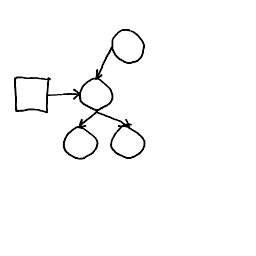
\includegraphics[width = \exampleImageSize]{figures/expert-60.png}&
  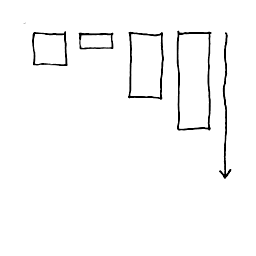
\includegraphics[width = \exampleImageSize]{figures/expert-5.png}&
    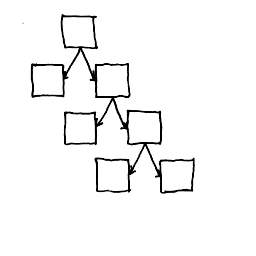
\includegraphics[width = \exampleImageSize]{figures/expert-17.png}&
    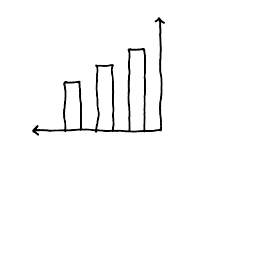
\includegraphics[width = \exampleImageSize]{figures/expert-58.png}\\
  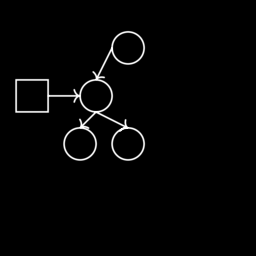
\includegraphics[width = \exampleImageSize]{figures/60.png}&
  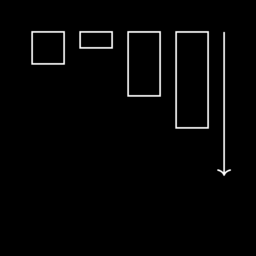
\includegraphics[width = \exampleImageSize]{figures/5.png}&
    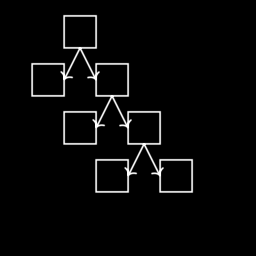
\includegraphics[width = \exampleImageSize]{figures/17.png}&
    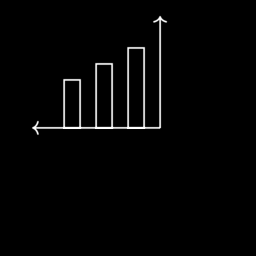
\includegraphics[width = \exampleImageSize]{figures/58.png}
\end{tabular}
\subcaption{}
  \end{minipage}%
  \begin{minipage}[t]{0.3\linewidth}
    \begin{tikzpicture}
      \node(picture) at (0,0) {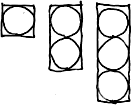
\includegraphics[width = 2cm]{figures/expert-31.png}};
      \draw[very thick,->] (picture.south)  -- (0,-2);
    \end{tikzpicture}\\
    \begin{minipage}[t]{0.3\linewidth}
\begin{Verbatim}
for (i < 3)
 rectangle(3*i,-2*i+4,
           3*i+2,6)
 for (j < i + 1)
  circle(3*i+1,-2*j+5)
\end{Verbatim}      
      \end{minipage}
    \subcaption{}
  \end{minipage}
  \caption{(a): Model learns to convert hand drawings (top) into \LaTeX~(rendered below). (b) Synthesizes high-level \emph{graphics program} from hand drawing.}\label{firstPageExamples}
\end{figure}
 
The key observation behind our work is that generating a programmatic representation from an image of a diagram  involves two distinct steps that require different technical approaches. The first step involves identifying the components such as rectangles, lines and arrows that make up the image. The second step involves identifying the high-level structure in how the components were drawn. In Fig. 1(b), it means identifying a pattern in how the circles and rectangles are being drawn that is best described with two nested loops, and which can easily be extrapolated to a bigger diagram. 

We present a hybrid architecture for inferring graphics programs that is structured around these two steps. For the first step,   a deep network to infers a set of primitive shape-drawing commands. We refer to this set as a \emph{trace set} since it corresponds to the set of commands in a program's execution trace but lacks the high-level structure that determines how the program decided to issue them.
%For added robustness, we train the network to produce a proposal distribution of the most likely traces and use stochastic search to find the trace that best matches the image.
%The network is trained from an automatically-generated corpus of synthetic image-generating programs.
The second step involves synthesizing a high-level program capable of producing the trace set identified by the first phase.
%In principle, we could also train a neural network to learn this mapping. In practice, though, this would be challenging because it would no longer be sufficient to train the network with a synthetic corpus of randomly generated programs, since our goal is to generate programs that satisfy certain semantic constraints that ensure that we get the program that the user most likely intended.
%This paper argues that this stage is best
We achieve this by \emph{constraint-based program synthesis} \citep{solar2008program}. The program synthesizer searches the space of possible programs for one capable of producing the desired trace set -- inducing structures like
symmetries, loops, or conditionals.
Although these program synthesizers do not need any training data,
we show how to learn a \emph{search policy} 
in order to synthesize programs an order of magnitude faster than constraint-based synthesis techniques alone.

One might be tempted to try to go directly from perceptual input (an image) to a program,
much like recent neural models of program induction that regress from problem statements to programs (e.g.,~\cite{devlin2017robustfill}). We advocate an alternative framing, which we call The Trace Hypothesis:

%% Images are high-dimensional and unstructured while programs are high-level
%% and symbolic. We resolve this mismatch by advancing a new model of
%% collaboration between these two representations, which we call The Trace Hypothesis:

\noindent \textbf{The Trace Hypothesis.} The set of commands issued by a program,
which we call a \emph{trace set},
is the correct liaison between high-dimensional unstructured perceptual input and high-level structured symbolic representations.

The roadmap of our paper is structured around the trace hypothesis, as outlined in Fig.~\ref{roadmap}.
\begin{figure}[h]
  \centering\begin{tikzpicture}
    \node[ thick,anchor = west,inner sep=0pt,label=below:{\small Perceptual input}](observation) at (0,0) {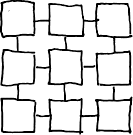
\includegraphics[width = 1.5cm]{figures/expert-39-trimmed.png}};
    \node[ultra thick,anchor = west,inner sep=0pt](traceSource) at (3,0.5){    \begin{lstlisting}[basicstyle = \scriptsize\ttfamily]
line, line,
rectangle,
line, ...
\end{lstlisting}};
    \node[ultra thick,anchor = west,inner sep=0pt](traceImage) at (3.3,-0.5) {
      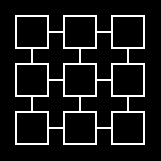
\includegraphics[width = 0.9cm]{figures/39-parse.png}}; 
    \node(trace)[draw,thin,fit = (traceImage) (traceSource), label = below:{{\small Trace set}}] {};
    
    \node[draw, thick,anchor = west,inner sep=2pt,label=below:{\small Program}](program) at (6.3,0) {
      \begin{lstlisting}
for (j < 3)
for (i < 3)
if (...)
 line(...)
 line(...)
rectangle(...)
    \end{lstlisting}};
    \node[ultra thick,anchor = west,inner sep=0pt,label=below:{\small Extrapolation}](extrapolate) at (9.9,-0.4) {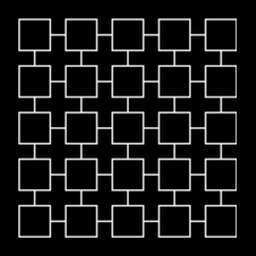
\includegraphics[width = 1.3cm]{figures/39-extrapolated.png}};
%    \node[ultra thick,anchor = west,inner sep=0pt,label=below:{\small Similarity}](similarity) at (11.3,0) {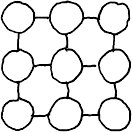
\includegraphics[width = 1cm]{figures/expert-38-trim.png}};
    \node[ultra thick,anchor = west,text width = 1.3cm,inner sep=0pt](errors) at (10,1) {\small Error correction};

    \draw[->, thick] (observation.east) -- node[draw,fill = white,rotate = -90] {{\small Neural network}} (trace.west);
    \draw[->, thick] (trace.east) -- node[draw,fill = white,rotate = -90] {{\small Program synthesis}} (program.west);
    \draw[->, thick] (program.east) to[out = 80,in = 180] (errors.west);
%    \draw[->, thick] (program.east) to[out = 40,in = -230] (similarity.west);
        \draw[->, thick] (program.east) to[out = -90,in = 180] (extrapolate.west);

    \draw[decoration = {brace,mirror,raise = 5pt},decorate,thick]
    ([yshift = -15,xshift = -115]trace.south) -- node[below = 6pt] {{\small Section~\ref{neuralNetworkSection}: Perception$\to$Trace set}} ([yshift = -15,xshift = -5]trace.south);
    \draw[decoration = {brace,mirror,raise = 5pt},decorate,thick]
    ([xshift = 5,yshift = -15]trace.south) -- node[below = 6pt] {{\small Section~\ref{programSynthesisSection}: Trace Set$\to$Program}} ([xshift = 140,yshift = -15]trace.south);
    \draw[decoration = {brace,mirror,raise = 5pt},decorate,thick]
([xshift = 150,yshift = -15]trace.south) -- node[below = 6pt] {{\small Section~\ref{applicationsSection}: Applications}} ([xshift = 230,yshift = -15]trace.south);
  \end{tikzpicture}
  \caption{Both the paper and the system pipeline are structured around the \emph{trace hypothesis}}\label{roadmap}
\end{figure}

The new contributions of this work are:
(1) The trace hypothesis: a framework for going from perception to programs,
which connects this work to other trace--based models,
like the  Neural Program Interpreter~\citep{DBLP:journals/corr/ReedF15};
(2) A model based on the trace hypothesis that converts sketches to high-level programs:
in contrast to converting images to vectors or low-level parses~\citep{huang2017shape,Nishida:2016:ISU:2897824.2925951,nsd,DBLP:journals/corr/Beltramelli17,im2latex}.
(3) A generic algorithm for learning a policy for efficiently searching for programs,
building on Levin search~\citep{levin1973universal}
and recent work like DeepCoder~\citep{BalGauBroetal16}.

Even with the high-level idea of a trace set, going from hand drawings to programs remains difficult. We address  these challenges:
(1) Inferring trace sets from images requires \emph{domain-specific} design choices from the deep learning and computer vision toolkits (Sec.~\ref{neuralNetworkSection}). (2) Generalizing to noisy hand drawings, we will show, requires learning a \emph{domain-specific} noise model that is invariant to the variations across hand drawings (Sec.~\ref{generalizingTheHandDrawings}).  (3) Discovering good programs requires solving a difficult combinatorial search problem, because the programs are often long and complicated (e.g., 9 lines of code, with nested loops and conditionals). We give a \emph{domain-general} framework for learning a search policy that quickly guides program synthesizers toward the target programs (Sec.~\ref{learningASearchPolicy}).

  

%under a quantitative objective that maximizes the likelihood according to a prior distribution that aims to capture the user’s preference.

%% The key observation behind our work is that generating a programmatic representation from an image of a diagram actually involves two distinct steps that require different technical approaches. The first step involves identifying the components such as boxes, lines and arrows that make up the image. The second step involves identifying the high-level structure in how the components were drawn; for example, in Fig. 1(b), it means identifying that there is a pattern in how the circles and rectangles are being drawn that is best described with two nested loops, and which can easily be extrapolated to a bigger diagram. 

%% We present a hybrid architecture for inferring graphics programs that is structured around these two steps. For the first step, our approach uses a deep neural network to infer a sequence of primitive shape-drawing commands that can generate an image similar to the observed image. We refer to this sequence as an \emph{execution trace}, since it corresponds to the sequence of primitive commands that the desired program would have issued, but it lacks the high-level structure that determines how the program decided to issue those commands. For added robustness, we train the network to produce a proposal distribution of the most likely traces, and use stochastic search to find the trace that best matches the input. The network is trained from an automatically generated corpus of synthetic image generating programs. 


%% High dimensional perceptual input may seem ill matched to the abstract
%% semantics of a programming language. But programs with constructs such as
%% recursion or iteration produce a simpler \emph{execution trace} of
%% primitive actions; for our domain, the primitive actions are drawing
%% commands. Our hypothesis is that the execution trace of the program is
%% better aligned with the perceptual input, and that the trace can act
%% as a kind of bridge between perception and programs. We test this
%% hypothesis by developing a model that learns to map from an image to
%% the execution trace of the graphics program that drew it.  With the
%% execution trace in hand, we can bring to bear techniques from the
%% program synthesis community to recover the latent graphics program.
%% This family of techniques, called \emph{constraint-based program synthesis}~\cite{solar2008program},
%% work by modeling a set of possible programs inside of a constraint solver,
%% such as a SAT or SMT solver~\cite{de2008z3}.
%% These techniques excel at uncovering high-level symbolic structure,
%% but are not well equipped to deal with real-valued perceptual inputs.


%% We develop a hybrid architecture for inferring graphics programs.  Our
%% approach uses a deep neural network infer an execution trace from an
%% image; this network recovers primitive drawing operations such as
%% lines, circles, or arrows, along with their parameters. For added
%% robustness, we use the deep network as a proposal distribution for a
%% stochastic search over execution traces.  Section~\ref{neuralNetworkSection} describes this first stage of the architecture where we infer drawing commands from images, and explains how we handle noisy hand drawings.
%% Finally, we use program synthesis techniques to recover the program from its
%% trace.  The program synthesizer discovers constructs such as loops and
%% geometric operations such as reflections and affine transformations.
%% % \remark{This paragraph is all about making things a bit more
%% Section~\ref{programSynthesisSection} describes how the architecture
%% synthesizes programs from execution traces,
%% and how those programs are used for  correcting errors made by the deep network, measuring similarity between hand drawings,
%% and extrapolating figures.


%   so you really need more specifics about program synth here.}

%% Each of these three components -- the deep network, the stochastic
%% search, the program synthesizer -- confers its own advantages. From
%% the deep network, we get a fast system that can recover plausible
%% execution traces in about a minute~\remark{A minute seems slow to me, for deep net inference...}. From the stochastic search, we get
%% added robustness: essentially, the stochastic search can correct
%% mistakes made by the deep network's proposals.  From the program
%% synthesizer, we get abstraction: our system recovers coordinate
%% transformations, for loops, and subroutines, which are useful for
%% downstream tasks and can help correct some mistakes of the earlier stages.
%% % \remark{I wonder if this would work even better as a bulleted list...}
%% \remark{Tie these claims into the paper results: state what the `downstream' tasks are that you actually do, and refer to the sections where they occur}




\section{Neural architecture for inferring trace sets}\label{neuralNetworkSection}

We developed a deep network architecture for efficiently inferring a
trace set, $T$, from an image, $I$.
Our model combines ideas from
Neurally-Guided Procedural Models~\citep{ritchie2016neurally}
and Attend-Infer-Repeat~\citep{eslami1603attend}.
The network constructs the
trace set one drawing command at a time, conditioned on what it has drawn so far.
%When predicting the next drawing
%command, the network takes as input the target image $I$ as well as
%the rendered output of previous drawing commands.
%Intuitively, the network looks at the image it wants to explain, as well as what it has already drawn.  It then decides either to stop drawing or proposes another drawing command to add to the trace set; if it decides to continue drawing, the predicted primitive is rendered to its ``canvas'' and the process repeats.
Fig.~\ref{architecture} illustrates this architecture.  We first
pass a $256\times 256$ target image and a rendering of the trace set so
far (encoded as a two-channel image) to a convolutional network. Given
the features extracted by the convnet, a multilayer perceptron then
predicts a distribution over the next drawing command to add to the
trace set (see Tbl.~\ref{drawingCommandTable}).
%We predict the drawing command token-by-token,
%\footnote{Tokens are atomic symbols in the programming language  -- so the model is \emph{not} predicting lines of code character-by-character, but instead the model knows about the syntactic structure of primitive drawing commands}
%%   conditioning each token both on the image
%% features and on the previously generated tokens. 
We also use a
differentiable attention mechanism (Spatial Transformer
Networks:~\cite{jaderberg2015spatial}) to let the model attend to
different regions of the image while predicting drawing commands.
%In Fig.~\ref{architecture} the network first decided to emit the \verb|circle| token
%conditioned on the image features, then it emitted the $x$ coordinate of
%the circle conditioned on the image features and the \verb|circle|
%token, and finally it predicted the $y$ coordinate of the circle
%conditioned on the image features, the \verb|circle| token, and the
%$x$ coordinate.
We currently constrain
coordinates to lie on a discrete $16\times 16$ grid,
but the grid could be made arbitrarily fine.  %% See supplement for the full details
%% of the architecture, which we implemented in
%% Tensorflow~\citep{tensorflow2015-whitepaper}.
%% \remark{There are some more details that are important to provide
%%   about this architecture in the supplement: the
%%   functional form(s) of the probability distributions over tokens, the
%%   network layer sizes, which MLPs share parameters, etc.}

\tikzset{>=latex}
\begin{figure}[t]
  \begin{tikzpicture}
  \node[draw,blue,ultra thick,anchor = west,inner sep=0pt,label=below:Target image: $I$](observation) at (0,-1) {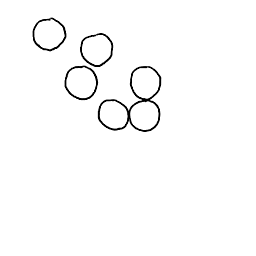
\includegraphics[width = 2cm]{figures/expert-18.png}};
  \node[draw,blue,thick,anchor = west,inner sep=0pt,minimum width = 2cm,minimum height = 2cm,label=below:Canvas: render$(T)$] (canvas) at (0,-4) {};
  \draw[lightgray,ultra thin,step = 0.125] ([xshift = 0.5,yshift = 0.5]canvas.south west) grid ([xshift = -0.5,yshift = -0.5]canvas.north east);
  % draw partial image on canvas
  \draw (0.375cm,-3.25cm) circle (0.125cm);
  \draw (0.625cm,-3.625) circle (0.125cm);
  \draw (0.75cm,-3.375) circle (0.125cm);

  \node[draw,ultra thick,anchor = west,inner sep=0pt,minimum width = 2cm,minimum height = 3cm] (CNN) at (4.5,-2.5) {CNN};
  \node[inner sep = 0pt](tensorProduct) at ([xshift = -1.5cm]CNN.west) {$\bigoplus$};

  \node[rotate = -90,draw,ultra thick,inner sep=0pt,minimum width = 3cm,minimum height = 0.5cm] (features) at ([xshift = 1.5cm]CNN.east) {Image features};

  \node[draw,ultra thick,minimum size = 1cm](c1) at ([xshift = 1.5cm]features.north) {MLP};
  \node(l1) at ([yshift = -1.5cm]c1.south) {\verb|circle(|};
  \node[draw,ultra thick,minimum size = 1cm](a2) at ([xshift = 1cm,yshift = 1.5cm]c1.east) {STN};
  \node[draw,ultra thick,minimum size = 1cm](c2) at ([xshift = 1cm]c1.east) {MLP};
  \draw[->,ultra thick] (a2.south) -- (c2.north);
  \draw[->,ultra thick,red] (c1.south) -- (l1.north);
  \node(l2) at ([yshift = -1.5cm]c2.south) {\verb|X=7,|};
  \draw[->,ultra thick,red] (c2.south) -- (l2.north);
  \node[draw,ultra thick,minimum size = 1cm](a3) at ([xshift = 1cm,yshift = 1.5cm]c2.east) {STN};
  \node[draw,ultra thick,minimum size = 1cm](c3) at ([xshift = 1cm]c2.east) {MLP};
  
  \draw[->,ultra thick] (a3.south) -- (c3.north);
  \node(l3) at ([yshift = -1.5cm]c3.south) {\verb|Y=12)|};
  \draw[->,ultra thick,red] (c3.south) -- (l3.north);

  
  \draw[->,ultra thick] (features.north) -- (c1.west);
  \draw[->,ultra thick] (features.north) to[out = 45,in = 160] (a2.north);
  \draw[->,ultra thick] (features.north) to[out = 70,in = 140] (a3.north);
  \draw[->,ultra thick] ([xshift = 0.25cm]l1.north) -- (c2.west);
  \draw[->,ultra thick] ([xshift = 0.25cm]l1.north) -- ([yshift = -0.2cm]c3.west);
  \draw[->,ultra thick] ([xshift = 0.25cm]l2.north) -- ([yshift = -0.25cm]c3.west);

  \node(next)[draw,very thick,fit = (l1) (l2) (l3), dashed, label = below:{Next drawing command}] {};

  \draw[-{>[scale = 1.5]},very thick,dashed] (next.west) -- ([yshift = -0.2cm]canvas.east) node [midway, below, sloped] (TextNode) {Renderer}; %: \LaTeX~Ti\emph{k}Z};
  
  \draw[->,ultra thick] (canvas.east) -- (tensorProduct.south);%[yshift = -0.5cm]CNN.west);
  \draw[->,ultra thick] (observation.east) -- (tensorProduct.north);%([yshift = 0.5cm]CNN.west);
  \draw[->,ultra thick] (tensorProduct.east)  -- node[fill = white,rotate = 90] {{\tiny $256\times 256\times 2$}}  (CNN.west);
  \draw[->,ultra thick] (CNN.east) -- node[fill = white,rotate = 90] {{\tiny $16\times 16\times 10$}} (features.south);
%  \draw[]
  
%  \node at (canvas.x,canvas.y) {Canvas};
\end{tikzpicture}
\caption{Our neural architecture for inferring the trace set of a graphics program from its output. \textcolor{blue}{Blue}: network inputs. Black: network operations. \textcolor{red}{Red}: samples from a multinomial. \texttt{Typewriter font}: network outputs. Renders snapped to a $16\times 16$ grid, illustrated in \textcolor{gray}{gray}. STN (spatial transformer network) is a differentiable attention mechanism~\citep{jaderberg2015spatial}.}  \label{architecture}
\end{figure}
\begin{table}[t]
  \caption{Primitive drawing commands currently supported by our model.}
\label{drawingCommandTable}
\begin{tabular}{ll}\toprule
  \begin{tabular}{l}
    \verb|circle|$(x,y)$
  \end{tabular}& \begin{tabular}{l}
    Circle at $(x,y)$
    \end{tabular}\\
  \begin{tabular}{l}
    \verb|rectangle|$(x_1,y_1,x_2,y_2)$
  \end{tabular}&\begin{tabular}{l}
    Rectangle with corners at $(x_1,y_1)$ \& $(x_2,y_2)$
    \end{tabular}\\
  \begin{tabular}{l}
    \verb|line|$(x_1,y_1,x_2,y_2,$\\
    \hspace{1cm}$\text{arrow}\in\{0,1\},\text{dashed}\in\{0,1\})$
  \end{tabular}&\begin{tabular}{l}
    Line from $(x_1,y_1)$ to  $(x_2,y_2)$,\\\hspace{1cm}optionally with an arrow and/or dashed
    \end{tabular}\\
  \begin{tabular}{l}
    \verb|STOP|
  \end{tabular}&\begin{tabular}{l}
    Finishes trace set inference
    \end{tabular}
\\  \bottomrule
\end{tabular}
\end{table}



%% For the model in Fig.~\ref{architecture}, the distribution over the next drawing command factorizes as:
%% \begin{equation}
%%   \probability_\theta [t_1t_2\cdots t_K | I,T] = \prod_{k = 1}^K \probability_\theta \left[t_k | a_\theta \left(f_\theta(I,\text{render}(T)) | \{t_j\}_{j = 1}^{k - 1}\right), \{t_j\}_{j = 1}^{k - 1}\right]
%% \end{equation}
%% where $t_1t_2\cdots t_K$ are the tokens in the drawing command, $I$ is
%% the target image, $T$ is a trace set, $\theta$ are the
%% parameters of the neural network, $f_\theta(\cdot,\cdot)$ is the
%% image feature extractor (convolutional network), and $a_\theta(\cdot|\cdot)$ is an attention mechanism. The distribution over
%% traces factorizes as:
%% \begin{equation}
%%   \probability_\theta [T|I] = \prod_{n = 1}^{|T|} \probability_\theta [T_n | I,T_{1:(n-1)}]\times\probability_\theta [\verb|STOP| | I,T]\label{objective}
%% \end{equation}
%% where $|T|$ is the length of trace set $T$, the subscripts
%% on $T$ index drawing commands within the trace (so $T_n$ is a sequence of tokens: $t_1t_2\cdots t_K$), and the \verb|STOP|
%% token is emitted by the network to signal that the trace set
%% explains the image.
We train the network by sampling trace sets $T$ and target
images $I$ for randomly generated scenes
and maximizing
%Eq.~\ref{objective}
 the likelihood of $T$ given $I$ with respect to
 the model parameters, $\theta$,
  by gradient ascent.
We trained the network on $10^5$ scenes, which takes a day on an Nvidia TitanX GPU.

%% Training does not require backpropagation across the sequence
%% of drawing commands: drawing to the canvas `blocks' the gradients,
%% effectively offloading memory to an external visual store.  
%% This approach is like an autoregressive version of
%% Attend-Infer-Repeat~\citep{eslami1603attend}, but critically, without a learned
%%   recurrent memory state, e.g. an RNN.  We can do without an RNN
%% because we learn from ground truth (image, trace) pairs.  This
%% allows us to handle scenes with many objects without
%% worrying about the conditioning of gradients as they propagate
%% over long sequences, and makes training more straightforward: it
%% is just maximum likelihood estimation of the model parameters.


\begin{wrapfigure}{r}{8cm}
  \vspace{-0.25cm}
  \centering
      \includegraphics[width = 7cm]{figures/averageNumberOfErrors.png}
      \caption{Parsing~\LaTeX~output after training on diagrams with $\leq 12$ objects. Model generalizes to scenes with many more objects. Neither SMC nor the neural network are sufficient on their own. \# particles varies by model: we compare the models \emph{with equal runtime} ($\approx 1$ sec/object)}\label{syntheticResults}\vspace{-0.7cm} 
\end{wrapfigure}
Our network can ``derender'' random synthetic images
%those shown in Fig.~\ref{trainingData}.
by doing a beam search to
recover  trace sets maximizing $\probability_\theta
[T|I]$. But, if the network predicts an incorrect
drawing command, it has no way of recovering from that error.  
%To derender an image with $n$ objects, it must correctly predict $n$ commands -- so its probability of success will decrease exponentially in $n$, assuming it has a nonzero chance of making a mistake.
For added robustness % as $n$ becomes large,
we treat the
 network outputs as proposals for a Sequential Monte Carlo (SMC) sampling scheme~\citep{SMCBook}.
%For the SMC sampler, we use pixel-wise distance as a surrogate for a likelihood function.
The SMC sampler is designed to sample
from the distribution $\propto L(I|\text{render}(T))
\probability_\theta[T|I]$, where $L(\cdot | \cdot)$
%:\text{image}^2\to\mathbb{R}$
uses the pixel-wise distance between two images as a proxy for a
likelihood.
Here, the network is learning a proposal distribution in an amortized way~\citep{paige2016inference}
and using it to invert a generative model (the renderer).
%% Unconventionally, the target distribution of the SMC sampler
%% includes the likelihood under the proposal distribution.
%% Intuitively, both the proposal
%% distribution and the distance function offer complementary signals for
%% whether a drawing command is correct.


\textbf{Experiment 1: Figure~\ref{syntheticResults}.}
  To evaluate which components of the model are necessary to parse complicated scenes,
  we compared  the neural network
  with SMC against the neural network by
itself or SMC by itself.  Only the combination of the two passes a
critical test of generalization: when trained on images with $\leq 12$
objects, it successfully parses scenes with many more objects than the
training data.
We compare with a baseline that produces the trace set in one shot by
using the CNN to extract features of the input which are passed to an LSTM which finally predicts
the trace set token-by-token (LSTM in Fig.~\ref{syntheticResults}).
This architecture is used in several successful neural models of image captioning (e.g.,~\cite{vinyals2015show}),
but, for this domain, cannot parse cluttered scenes with many objects.



%% \begin{figure}[H]\centering
%%   \begin{minipage}{6cm}
%%     \begin{minipage}[t]{3cm}\fbox{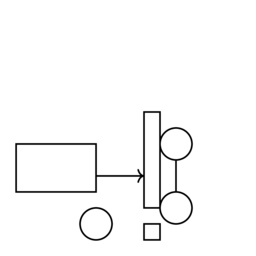
\includegraphics[width=2.75cm]{figures/randomScene-58-7.png}}\end{minipage}%
%%     \begin{minipage}[t]{3cm}\fbox{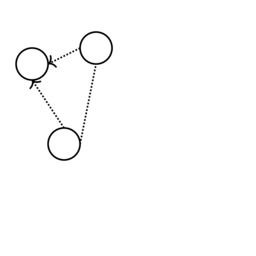
\includegraphics[width=2.75cm]{figures/randomScene-33-5.png}}\end{minipage}
%%     \caption{Network is trained to infer traces for randomly generated scenes like the two shown above. See supplement for details of the training data generation.}\label{trainingData}
%%   \end{minipage}\hfill%
%%   \begin{minipage}{7.5cm}\centering
%%     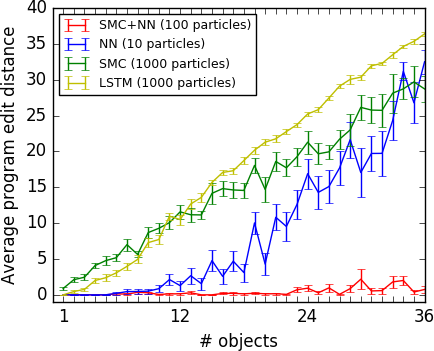
\includegraphics[width = 7cm]{figures/editDistance36.png}
%% %    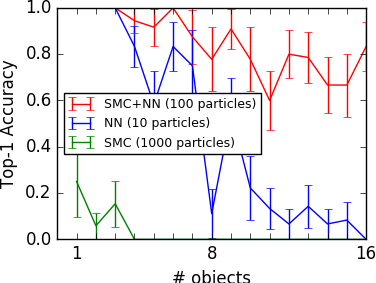
\includegraphics[width = 4cm]{figures/accuracy.png}
%%       \caption{Parsing~\LaTeX~output after training on diagrams with $\leq 12$ objects. It generalizes to scenes with many more objects. Neither the stochastic search nor the neural network are sufficient on their own. \# particles varies by model: we compare the models \emph{with equal runtime} ($\approx 1$ sec/object)}\label{syntheticResults}
%%     \end{minipage}
  
%%   \end{figure}

\subsection{Generalizing to real hand drawings}\label{generalizingTheHandDrawings}
%% \begin{wrapfigure}{R}{6cm}
%% \centering\vspace{-0.7cm}  \begin{minipage}[t]{2.5cm}\centering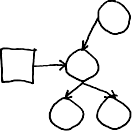
\includegraphics[width = 2cm]{figures/expert-60-reduced.png}
%%     \subcaption{}
%%   \end{minipage}\\
%%    \begin{minipage}[t]{2.5cm}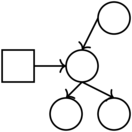
\includegraphics[width = 2cm]{figures/60-groundTruth-reduced.png}
%%     \subcaption{}
%%   \end{minipage}%
%%   \begin{minipage}[t]{2.5cm}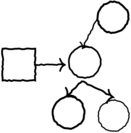
\includegraphics[width = 2cm]{figures/60-1-reduced.png}
%%     \subcaption{}
%%   \end{minipage}%
%%     \caption{(a): hand drawing. (b): Rendering of the trace set our model infers for (a). (c): noisy rendering of (b).}\label{handDrawingExamples}
%% \end{wrapfigure}

%A practical application of our neural network is the automatic conversion of hand drawings into a subset of \LaTeX.
 We trained the model
to generalize to hand drawings by introducing noise into the
renderings of the training target images.
We designed this noise process to introduce the kinds of variations found in hand drawings (%% Fig.~\ref{handDrawingExamples}; 
see supplement for details).

Our neurally-guided SMC procedure
used pixel-wise distance as a surrogate for a likelihood function ($L(\cdot|\cdot)$ in section~\ref{neuralNetworkSection}).
But pixel-wise distance fares poorly on hand drawings, which never exactly match
the model's renders.
So, for hand drawings,
we learn a surrogate likelihood function,
$L_{\text{learned}}(\cdot|\cdot)$.
The density $L_{\text{learned}}(\cdot|\cdot)$ is predicted by a convolutional network that we train to predict
the distance between two trace sets conditioned upon their renderings.
We train our likelihood surrogate to approximate the symmetric difference,
which is  the number of drawing commands by which two trace sets  differ:
  \begin{equation}
    -\log L_{\text{learned}}(\text{render}(T_1)|\text{render}(T_2))\approx |T_1 - T_2| + |T_2 - T_1|\label{symmetricDistance}
    \end{equation}



%% Pixel-wise distance metrics are sensitive to the details of how
%% arrows, dashes, and corners are drawn -- but we wish to be invariant
%% to these details.
%% So, we learn a distance metric over images that
%% approximates the distance metric in the search space over traces.

  \textbf{Experiment 2: Figures~\ref{drawingSuccesses}--\ref{drawingIntersectionOverUnion}.}
    We evaluated, but did not train, our system on 100 real hand-drawn figures; see Fig.~\ref{drawingSuccesses}--\ref{drawingFailures}.
These were drawn carefully but not perfectly with the aid of graph paper.
%Because our model assumes that objects are snapped to a $16\times 16$ grid, 
%we made the drawings on graph paper.
For each drawing we annotated a ground truth trace set and had the neurally guided SMC sampler
produce $10^3$ samples. % for each drawing.
For 63\% of the drawings, the Top-1 most likely sample exactly matches the
ground truth; with more samples, the model finds trace sets
that are closer to the ground truth annotation (Fig.~\ref{drawingIntersectionOverUnion}).
We will show that the program synthesizer
corrects some of these small errors (Sec.~\ref{synthesizerHelpsParsing}).
%% Because the model sometimes makes mistakes % on hand drawings,
%% we envision it working as follows:
%% a user sketches a diagram,
%% and the system responds by proposing a few candidate interpretations.
%% The user could then select the one closest to their intention and edit it if necessary.

\setlength\tabcolsep{3.5pt}
\begin{figure}[H]
  \begin{minipage}[t]{8.25cm}
    \begin{tabular}{llll}
      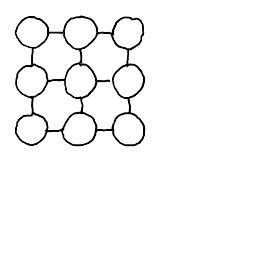
\includegraphics[width = 2cm]{figures/expert-38.png}&
      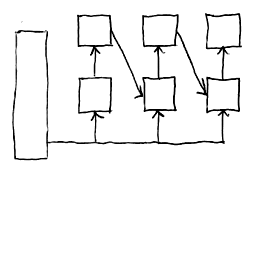
\includegraphics[width = 2cm]{figures/expert-73.png}&
      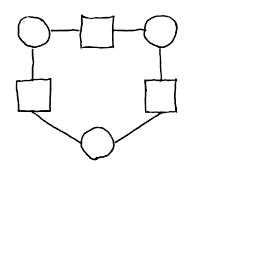
\includegraphics[width = 2cm]{figures/expert-77.png}&
      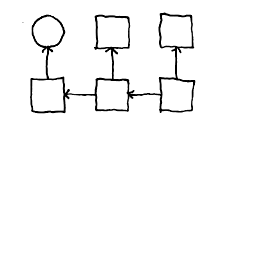
\includegraphics[width = 2cm]{figures/expert-21.png}
      \\
      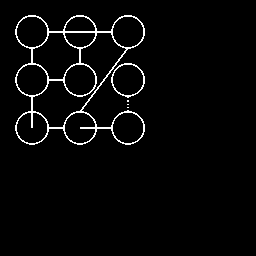
\includegraphics[width = 2cm]{figures/38-parse.png}     &
      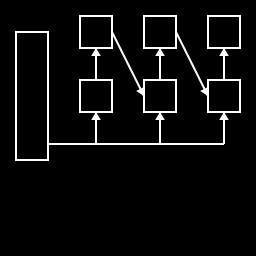
\includegraphics[width = 2cm]{figures/73-parse.png}     &
      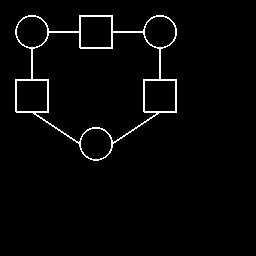
\includegraphics[width = 2cm]{figures/77-parse.png}    &
      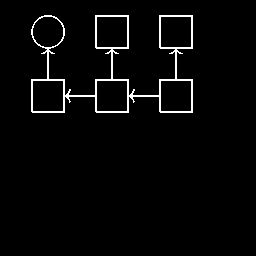
\includegraphics[width = 2cm]{figures/21-parse.png}    
      \end{tabular}
    \caption{Left to right: Ising model, recurrent network architecture, figure from a deep learning textbook \cite{Goodfellow-et-al-2016}, graphical model}\label{drawingSuccesses}
  \end{minipage}
\hfill  \begin{minipage}[t]{4.25cm}
    \begin{tabular}{ll}
          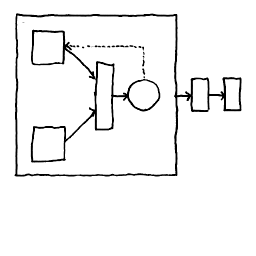
\includegraphics[width = 2cm]{figures/expert-1.png}&
          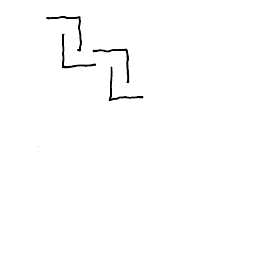
\includegraphics[width = 2cm]{figures/expert-34.png}\\
      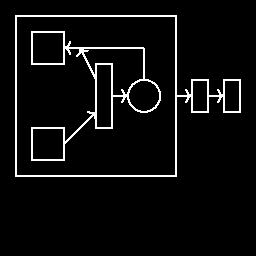
\includegraphics[width = 2cm]{figures/expert-1-parse.png}     &
              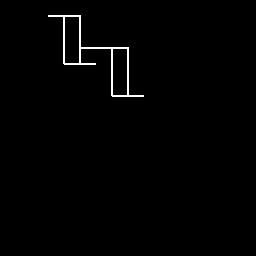
\includegraphics[width = 2cm]{figures/34-parse.png}    
    \end{tabular}


    \caption{Near misses. Rightmost: illusory contours (note: no SMC)}\label{drawingFailures}
  \end{minipage}


%  \caption{Example drawings above model outputs. See also Fig.~\ref{firstPageExamples}. Stochastic search (SMC) can help correct for these errors, as can the program synthesizer (Section~\ref{synthesizerHelpsParsing})}\label{lotsOfHandDrawings}
\end{figure}
\setlength\tabcolsep{6pt}

\begin{figure}[h]\centering
  \begin{minipage}[c]{0.57\textwidth} 
    \centering  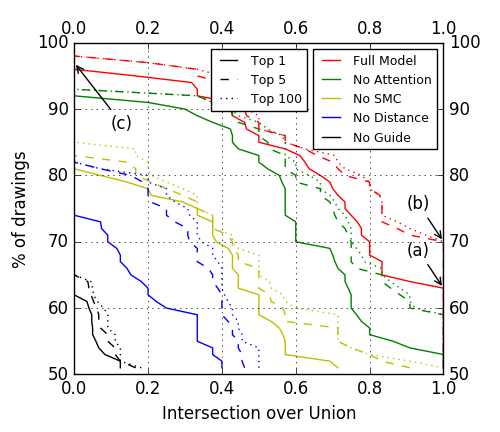
\includegraphics[width = 8cm]{figures/drawingAccuracy.png}            \vspace{-0.5cm}
  \end{minipage}\hfill%
      \begin{minipage}[c]{0.4\textwidth} 
  \caption{How close are the model's outputs to the ground truth on hand drawings, as we consider larger sets of samples (1, 5, 100)?
    Distance to ground truth trace set measured by the intersection over union (IoU) of predicted vs. ground truth: IoU of sets $A$ and $B$ is $|A\cap B|/|A\cup B|$. (a) for 63\% of drawings the model's top prediction is exactly correct; (b) for 70\% of drawings the ground truth is in the top 5 model predictions; (c) for 4\% of drawings all of the model outputs have no overlap with the ground truth. Red: the full model. Other colors: lesioned versions of our model.}\label{drawingIntersectionOverUnion}            \vspace{-0.5cm}
      \end{minipage}

\end{figure}

%\pagebreak





\section{Synthesizing graphics programs from trace sets}\label{programSynthesisSection}
Although the trace set of a graphics program describes the contents
of a scene, it does not encode higher-level features of the image,
such as repeated motifs or symmetries.  A \emph{graphics
  program} better describes such structures.
We seek to synthesize graphics programs from their trace sets.

We constrain the space of programs by writing down a context
free grammar over  programs -- 
%Although it might be desirable to synthesize programs in a Turing-complete language such as Lisp or Python, a more tractable approach is to specify
what in the program
languages community is called a Domain Specific Language (DSL)~\citep{polozov2015flashmeta}. Our DSL (Tbl.~\ref{DSL})
encodes prior knowledge of what graphics programs tend to look like.

\begin{table}[H]
  \caption{Grammar over graphics programs. We allow loops (\texttt{for}) with conditionals (\texttt{if}), vertical/horizontal reflections (\texttt{reflect}), variables (Var) and affine transformations ($\mathbb{Z}\times$Var\texttt{+}$\mathbb{Z}$).}\label{DSL}
  \begin{tabular}{rl}\toprule
  Program$\to$&Statement; $\cdots$; Statement\\
  Statement$\to$&\texttt{circle}(Expression,Expression)\\
  Statement$\to$&\texttt{rectangle}(Expression,Expression,Expression,Expression)\\
  Statement$\to$&\texttt{line}(Expression,Expression,Expression,Expression,Boolean,Boolean)\\
  Statement$\to$&\texttt{for}$(0\leq \text{Var}  < \text{Expression})$\texttt{ \{ if }$(\text{Var} > 0)$\texttt{ \{ }Program\texttt{ \}; }Program\texttt{ \}}\\
  Statement$\to$&\texttt{reflect}$(\text{Axis})$\texttt{ \{ }Program\texttt{ \}}\\
  Expression$\to$&$\mathbb{Z}\times$Var\texttt{+}$\mathbb{Z}$\\
%  Var$\to$&A free (unused) variable\\
  Axis$\to$&\texttt{X = }$\mathbb{Z}$ | \texttt{Y = }$\mathbb{Z}$\\
    $\mathbb{Z}\to$&an integer\\\bottomrule
  \end{tabular}
\end{table}

Given the DSL and a trace set $T$, we want a program that both evaluates to $T$
and, at the same time, is the ``best'' explanation of $T$.
For example, we might prefer more general programs or, in the spirit of Occam's razor,
prefer shorter programs.
We wrap these intuitions up into a cost function over programs,
and seek the minimum cost program consistent with $T$:
\begin{equation}
  \text{program}(T) = \argmin_{p\in \text{DSL, s.t. }p \text{ evaluates to } T} \text{cost}(p)\label{programObjective}
\end{equation}
We define the
cost of a program to be the number of Statement's it contains (Tbl.~\ref{DSL}).
We also penalize using many different numerical constants; see supplement.
%\remark{The flow here is a bit off/backwards. ``We want a program that evaluates to $T$ and also minimizes some measure of program cost''---why do we care about cost? It'd be better to start by making a ``Bayesian Occam's razor'' appeal (e.g. the most compact/general program is the more likely explanation) and then saying that one way to do this is to minimize a cost function which is proportional to program length.}

The constrained optimization problem in
Eq.~\ref{programObjective} is intractable in general, but there
exist efficient-in-practice tools for finding exact solutions to such
program synthesis problems. We use the state-of-the-art Sketch
tool~\citep{solar2008program}.
%At a high level,
Sketch takes as input a space of programs, along with
a specification of the program's behavior and optionally a cost
function.  It translates the synthesis problem into a constraint
satisfaction problem and then uses a SAT solver to find a minimum-cost
program satisfying the specification.  Sketch requires a
 \emph{finite program space}, which here means that the depth of the
program syntax tree is bounded (we set the bound to 3),
but has the guarantee that it 
always eventually finds a globally optimal solution.
In exchange for this optimality guarantee
it comes with no guarantees
on runtime.
For our domain synthesis times vary from minutes to hours,
with 27\% of the drawings timing out the synthesizer after 1 hour.
Tbl.~\ref{exampleSynthesisResults} shows programs recovered by our system.
A main impediment to our use of these general techniques is
the prohibitively high cost of searching for programs.
We next describe how to learn to synthesize programs much faster (Sec.~\ref{learningASearchPolicy}),
timing out on 2\% of the drawings and solving 58\% of problems within a minute.

\newcommand{\exampleProgramSize}{4cm}
\newcommand{\exampleTraceSize}{3.5cm}
\newcommand{\exampleDrawingSize}{1.25cm}
\lstset{basicstyle = \scriptsize\ttfamily}

\begin{table}[t]
  \caption{Example drawings (left), their ground truth trace sets (middle left), and programs synthesized from these trace sets (middle right). Compared to the trace sets the programs are more compressive (right: programs have fewer lines than traces) and automatically group together related drawing commands. Note the nested loops  and special case conditionals in the Ising model, combination of symmetry and iteration in the bottom figure,  affine transformations in the top figure, and the complicated program in the second figure to bottom.}\label{exampleSynthesisResults}
%  \vspace{-0.6cm}
\centering  \begin{tabular}{m{1.5cm}llc}
    \toprule
    \textbf{Drawing}&\textbf{Trace Set}&\textbf{Program}&%\begin{tabular}{c}
      \textbf{Compression factor}%\\\textbf{factor}
      %      \end{tabular}\\
      \\
    \midrule
    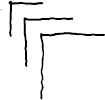
\includegraphics[width = \exampleDrawingSize]{figures/expert-29-trim.png}&
\begin{minipage}{\exampleTraceSize}\begin{lstlisting}
Line(2,15, 4,15)
Line(4,9, 4,13)
Line(3,11, 3,14)
Line(2,13, 2,15)
Line(3,14, 6,14)
Line(4,13, 8,13)
\end{lstlisting}
\end{minipage}&     \begin{minipage}{\exampleProgramSize} \begin{lstlisting}
for(i<3)
 line(i,-1*i+6,
      2*i+2,-1*i+6)
 line(i,-2*i+4,i,-1*i+6)
       \end{lstlisting}
     \end{minipage}&$\frac{6}{3} = 2\text{x}$\\\midrule
%%      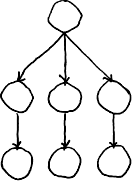
\includegraphics[width = \exampleDrawingSize]{figures/expert-52-trim.png}&
%% \begin{minipage}{\exampleTraceSize}\begin{lstlisting}
%% Line(5,13,2,10,arrow)
%% Circle(5,9)
%% Circle(8,5)
%% Line(2,8, 2,6,arrow)
%% Circle(2,5)
%% \end{lstlisting}
%% \small\emph{... etc. ...; 13 lines}
%% \end{minipage}&
%%              \begin{minipage}{\exampleProgramSize}\begin{lstlisting}
%% circle(4,10)
%% for(i<3)
%%  circle(-3*i+7,5)
%%  circle(-3*i+7,1)
%%  line(-3*i+7,4,-3*i+7,2,arrow)
%%  line(4,9,-3*i+7,6,arrow)
%% \end{lstlisting}
%% \end{minipage}&$\frac{13}{6} = 2.2\text{x}$\\\midrule
    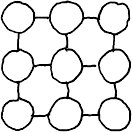
\includegraphics[width = \exampleDrawingSize]{figures/expert-38-trim.png}&
\begin{minipage}{\exampleTraceSize}\begin{lstlisting}
Circle(5,8)
Circle(2,8)
Circle(8,11)
Line(2,9, 2,10)
Circle(8,8)
Line(3,8, 4,8)
Line(3,11, 4,11)
\end{lstlisting}
  \small\emph{... etc. ...; 21 lines}
\end{minipage}&\begin{minipage}{\exampleProgramSize}
\begin{lstlisting}
for(i<3)
 for(j<3)
  if(j>0)
   line(-3*j+8,-3*i+7,
        -3*j+9,-3*i+7)
   line(-3*i+7,-3*j+8,
        -3*i+7,-3*j+9)
  circle(-3*j+7,-3*i+7)
\end{lstlisting}
\end{minipage}&$\frac{21}{6} = 3.5\text{x}$\\\midrule
\includegraphics[width = \exampleDrawingSize]{figures/expert-101-trim.png}&
\begin{minipage}{\exampleTraceSize}\begin{lstlisting}
Rectangle(1,10,3,11)
Rectangle(1,12,3,13)
Rectangle(4,8,6,9)
Rectangle(4,10,6,11)
\end{lstlisting}
  \small\emph{... etc. ...; 16 lines}
\end{minipage}&\begin{minipage}{\exampleProgramSize}
\begin{lstlisting}
for(i<4)
 for(j<4)
  rectangle(-3*i+9,-2*j+6,
            -3*i+11,-2*j+7)
\end{lstlisting}
\end{minipage}&$\frac{16}{3} = 5.3\text{x}$\\\midrule
%% 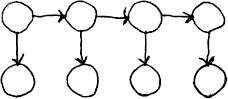
\includegraphics[width = \exampleDrawingSize]{figures/expert-75-extra-trim.png}&
%% \begin{minipage}{\exampleTraceSize}\begin{lstlisting}
%% Line(11,14,13,14,arrow)
%% Circle(10,10)
%% Line(10,13,10,11,arrow)
%% Circle(6,10)
%% \end{lstlisting}
%%     \small\emph{... etc. ...; 15 lines}
%% \end{minipage}&
%% \begin{minipage}{\exampleProgramSize}
%%     \begin{lstlisting}
%% for(i<4)
%%  line(-4*i+13,4,-4*i+13,2,arrow)
%%  for(j<3)
%%   if(j>0)
%%    circle(-4*i+13,4*j+-3)
%%   line(-4*j+10,5,-4*j+12,5,
%%        arrow)
%% \end{lstlisting}
%%   \end{minipage}&$\frac{15}{6} = 2.5\text{x}$\\\midrule    

  \includegraphics[width = \exampleDrawingSize]{figures/expert-71-trim.png}&
\begin{minipage}{\exampleTraceSize}\begin{lstlisting}
Line(3,10,3,14,arrow)
Rectangle(11,8,15,10)
Rectangle(11,14,15,15)
Line(13,10,13,14,arrow)
  \end{lstlisting}\small\emph{... etc. ...; 16 lines}%
  \end{minipage}&\begin{minipage}{\exampleProgramSize}
%% \begin{lstlisting}
%% for (i<3)
%%  circle(-3*i+7,1)
%%  circle(-3*i+7,6)
%%  line(-3*i+7,-1*i+4,-3*i+7,5)
%% \end{lstlisting}
\begin{lstlisting}
for(i<3)
 line(7,1,5*i+2,3,arrow)
 for(j<i+1)
  if(j>0)
   line(5*j-1,9,5*i,5,arrow)
  line(5*j+2,5,5*j+2,9,arrow)
 rectangle(5*i,3,5*i+4,5)
 rectangle(5*i,9,5*i+4,10)
rectangle(2,0,12,1)
\end{lstlisting}
\end{minipage}&$\frac{16}{9} = 1.8\text{x}$\\\midrule    

  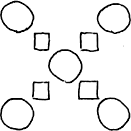
\includegraphics[width = \exampleDrawingSize]{figures/expert-72-trim.png}&

\begin{minipage}{\exampleTraceSize}\begin{lstlisting}
Circle(2,8)
Rectangle(6,9, 7,10)
Circle(8,8)
Rectangle(6,12, 7,13)
Rectangle(3,9, 4,10)
\end{lstlisting}\small\emph{... etc. ...; 9 lines}
  \end{minipage}&\begin{minipage}{\exampleProgramSize}
\begin{lstlisting}
reflect(y=8)
 for(i<3)
  if(i>0)
   rectangle(3*i-1,2,3*i,3)
  circle(3*i+1,3*i+1)
\end{lstlisting}
\end{minipage}&$\frac{9}{5} = 1.8\text{x}$ \\\bottomrule
  \end{tabular}
  \end{table}

\subsection{Learning a search policy for synthesizing programs}\label{learningASearchPolicy}

We want to leverage powerful, domain-general techniques from the program synthesis community,
but make them much faster by
learning a domain-specific \emph{search policy}.
A search policy poses search problems
like those in Eq.~\ref{programObjective},
but also offers additional constraints on the structure of the program (Tbl.~\ref{policyOutput}).
For example, a policy might decide to first try searching over small programs before searching over large programs,
or decide to prioritize searching over programs that have loops.

A search policy $\pi_\theta(\sigma  | T )$ takes as input a trace set $T$ and predicts a distribution over synthesis problems, each of which is written $\sigma $ and corresponds to a set of possible programs to search over (so $\sigma \subseteq \text{DSL}$).
Good policies will prefer tractable program spaces,
so that the search procedure will terminate early, 
but should also prefer program spaces likely to contain
programs that concisely explain the data.
These two desiderata are in tension:
tractable synthesis problems involve searching over smaller spaces,
but smaller spaces are less likely to contain good programs.
%a minimum cost program
%for explaining $T$.
Our goal now is to find the parameters of the policy, written $\theta$, which best navigate this trade-off.


Given a search policy, what is the best way of using it to quickly find minimum cost programs?
We use a \emph{bias-optimal search algorithm}~\citep{schmidhuber2004optimal}:

\noindent\textbf{Definition: Bias-optimality.} 
   A search algorithm is $n$-\emph{bias optimal}
with respect to a distribution $\probability_{\text{bias}}[\cdot ]$ if it is
guaranteed to find a solution in $\sigma $ after searching for at least time
$n\times\frac{t(\sigma )}{\probability_{\text{bias}}[\sigma ]}$, where $t(\sigma )$ is the time it
takes to verify that $\sigma $ contains a solution to the
search problem.




%Intuitively, an $n$-bias optimal search algorithm spends at least $\probability_{\text{bias}}[\sigma ]/n$ of its time exploring solution space $\sigma $.
An example of a $1$-bias optimal search algorithm is a time-sharing system that allocates $\probability_{\text{bias}}[\sigma ]$ of its time to trying $\sigma $. We construct a $1$-bias optimal search algorithm by identifying $\probability_{\text{bias}}[\sigma ] = \pi_\theta(\sigma |T)$ and $t(\sigma )  = t(\sigma|T)$, where $t(\sigma|T)$ is how long the synthesizer takes to search $\sigma $ for a program for $T$. This means that the search algorithm explores the entire program space, but spends most of its time in the regions of the space that  the policy judges to be most promising.


%% \begin{figure}\centering
%%   \begin{tikzpicture}
%%     \node[anchor = west] at (0,5.25) {Entire program search space};
%%     \draw[fill = yellow,fill opacity = 0.15,draw = black] (0,0) rectangle (5,5);
%%     \draw [fill = yellow, opacity = 0.2] (0,0)--(0,2)--(4,0)--(0,0);
%%     \draw [fill = yellow, opacity = 0.4,cycle] (0,5)--(0,1)--(3,5);
%%     \draw [fill = yellow, opacity = 0.6,cycle] (2.5,5)--(3.2,0)--(5,0)--(5,5);
%%     \draw (0,2) -- node[below,sloped]{short programs} (4,0);
%%     \draw (0,2) -- node[above,sloped]{long programs} (4,0);
%%     \draw (2.5,5) -- node[above,sloped]{programs w/ reflections} (3.2,0);
%%     \draw (0,1) -- node[above,sloped]{ programs w/ loops} (3,5);
%%     \node(p1)[anchor =west ] at (5.5,3.5) {$\pi_\theta(\text{short, no loop/reflect}) = $};
%%     \draw [fill = yellow, fill opacity = 0.2,draw = black]  ([xshift = 0cm,yshift = -0.2cm]p1.east) rectangle ([xshift = 0.4cm,yshift = 0.2cm]p1.east);
%%     \node(p2)[anchor =west ] at ([yshift = -0.5cm]p1.west) {$\pi_\theta(\text{long, loops}) = $};
%%     \draw [fill = yellow, fill opacity = 0.4,draw = black]  ([xshift = 0cm,yshift = -0.2cm]p2.east) rectangle ([xshift = 0.4cm,yshift = 0.2cm]p2.east);
%%     \node(p3)[anchor =west ] at ([yshift = -0.5cm]p2.west) {$\pi_\theta(\text{long, no loop/reflect}) = $};
%%     \draw [fill = yellow, fill opacity = 0.15,draw = black]  ([xshift = 0cm,yshift = -0.2cm]p3.east) rectangle ([xshift = 0.4cm,yshift = 0.2cm]p3.east);
%%     \node(p4)[anchor =west ] at ([yshift = -0.5cm]p3.west) {$\pi_\theta(\text{long, reflects}) = $};
%%     \draw [fill = yellow, fill opacity = 0.6,draw = black]  ([xshift = 0cm,yshift = -0.2cm]p4.east) rectangle ([xshift = 0.4cm,yshift = 0.2cm]p4.east);
%%     \node(p5)[anchor =west ] at ([yshift = -0.5cm]p4.west) {\emph{etc.}};
%%   \end{tikzpicture}
%%   \caption{The bias-optimal search algorithm divides the entire (intractable) program search space in to (tractable) program subspaces (written $\sigma $), each of which contains a restricted set of programs. For example, one subspace might be short programs which don't loop. The policy $\pi$ predicts a distribution over program subspaces. The weight that $\pi$ assigns to a subspace is indicated by it's yellow shading in the above figure.}
%%   \end{figure}
Now in theory any $\pi_\theta(\cdot |\cdot ) $ is a bias-optimal searcher.
But the actual runtime of the algorithm depends strongly upon
the bias $\probability_{\text{bias}}[\cdot ]$.
Our new approach is to learn $\probability_{\text{bias}}[\cdot ]$
by picking the policy minimizing the
expected bias-optimal time to solve a training corpus, $\mathcal{D}$, of graphics program synthesis problems:
\begin{align}
\textsc{Loss}(\theta ; \mathcal{D})& =  \expect_{T\sim\mathcal{D}}\left[ \min_{\sigma\in \text{\textsc{Best}}(T)}\frac{t(\sigma | T)}{\pi_\theta (\sigma | T)}\right] + \lambda \Vert\theta\Vert_2^2\label{policyLoss}\\
\text{where }  \sigma \in\text{\textsc{Best}}(T) &\text{ if  a minimum cost program for }T \text{ is in }\sigma .\nonumber %\text{cost}(\text{program}(p)) = \min_{p\in \sigma \text{, s.t. }p\text{ evaluates to }T} \text{cost}(p) \nonumber
\end{align}
Practically, bias optimality has now bought us the following: (1) a guarantee that the policy will always find the minimum cost program; and (2) a differentiable loss function for the policy parameters that takes into account the cost of searching, in contrast to e.g. DeepCoder~\citep{BalGauBroetal16}.

To generate a training corpus for learning a policy which minimizes this loss,
we synthesized minimum cost programs for each trace set of our hand drawings
and for each $\sigma $.
%Solving these
%\footnote{There are 100 the drawings and $2\times 2\times 2\times 3 = 24$ different values of $\sigma $}
%synthesis problems takes a little over a day on 40 CPUs.
%With the training set in hand we  %This loss is differentiable but nonconvex even if $\pi_{\theta}(\cdot |\cdot )^{-1}$ is convex.
We locally minimize this loss using gradient descent. % while annealing a softened minimum to the hard minimization equation~\ref{policyLoss}.
%See supplement for details.
Because we want to learn a policy from only $100$ hand-drawn diagrams,
we chose a simple low-capacity, bilinear model for a policy:
\begin{equation}
  \pi_{\theta}(\sigma |T)\propto \exp \left( \phi_{\text{params}}(\sigma )^\top\theta \phi_{\text{trace}}(T)\right)
\end{equation}
where $\phi_{\text{params}}(\sigma  )$ is a one-hot encoding of
the parameter settings of $\sigma $ (see Tbl.~\ref{policyOutput})
and $\phi_{\text{trace}}(T)$ extracts a few simple features of the trace set $T$;
see supplement for details.

\textbf{Experiment 3: Figure~\ref{policyEvaluation}.}
We compare synthesis times for our learned search policy
with two alternatives:
 \emph{Sketch}, which poses the
entire problem wholesale to the Sketch program synthesizer;
and an \emph{Oracle},
a policy which always picks the quickest to search $\sigma $
 also containing a minimum cost program.
Our approach improves upon Sketch by itself,
and comes close to the Oracle's performance.
One could never construct this Oracle,
because the agent does not know ahead of time which
$\sigma $'s contain minimum cost programs nor does it know how long each
$\sigma $ will take to search.
%The Oracle is an upper bound on the performance of any search policy.
With this learned policy in hand we can synthesize 58\% of programs within a minute.
\end{experiment}
\begin{table}[h]\centering
  \caption{Parameterization of different ways of posing the program synthesis problem. The policy learns to choose parameters likely to quickly yield a minimal cost program. We slightly abuse notation by writing $\sigma $ to mean an assignment to each of these parameters (so $\sigma $ assumes one of 24 different values) and to mean the set of programs selected by that parameterization (so $\sigma \subseteq \text{DSL}$)}\label{policyOutput}
  \begin{tabular}{lll}\toprule
  Parameter&Description&Range\\\midrule
  Loops?&Is the program allowed to loop?&$\{\text{True},\text{False}\}$\\
  Reflects?&Is the program allowed to have reflections?&$\{\text{True},\text{False}\}$\\
  Incremental?&Solve the problem piece-by-piece or all at once?&$\{\text{True},\text{False}\}$\\
  Maximum depth& Bound on the depth of the program syntax tree&$\{1,2,3\}$
  \\\bottomrule
  \end{tabular}
  \end{table}
\begin{figure}[h]
  \centering  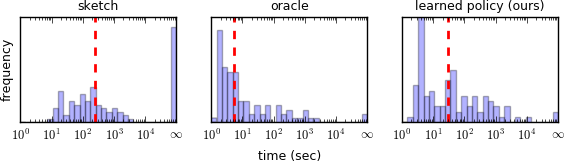
\includegraphics[width = 11cm]{figures/policyComparison.png}
  \caption{How long does it typically take to synthesize a minimum cost program? Sketch: out-of-the-box performance of the Sketch~\citep{solar2008program} program synthesizer. Oracle:  upper bounds  the performance of any search policy. Learned policy: a bias-optimal learned search policy running on an ideal timesharing machine.  $\infty = $ timeout. Red dashed line is median time. Learned policy evaluated using 20-fold cross validation.}\label{policyEvaluation}
\end{figure} 







\section{Applications of graphics program synthesis}\label{applicationsSection}
Why synthesize a graphics program,
if the trace set already suffices to recover the objects in an image?
Within our domain of hand-drawn figures, graphics program synthesis has several uses:

\pagebreak\subsection{Correcting errors made by the neural network}\label{synthesizerHelpsParsing}
\begin{wrapfigure}{r}{5cm}\vspace{-0.5cm}
  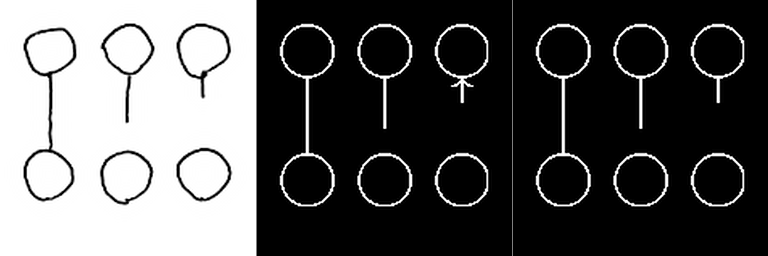
\includegraphics[width = 5cm]{figures/programSuccess7.png}
  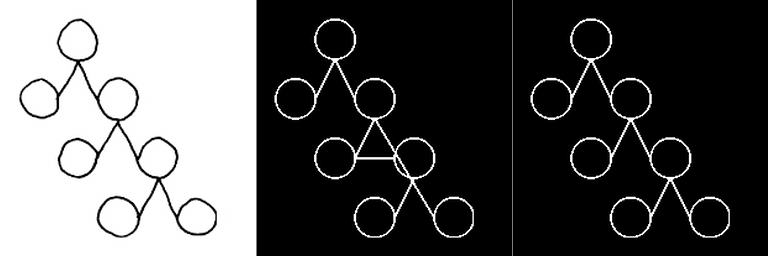
\includegraphics[width = 5cm]{figures/programSuccess16.png}
  \caption{Left: hand drawings. Center: interpretations favored by the deep network. Right: interpretations favored after learning a prior over programs. The prior favors  simpler programs, thus (top) continuing the pattern of not having an arrow is preferred, or (bottom) continuing the ``binary search tree'' is preferred.}\label{exampleOfProgramCorrectingMistake}
\vspace{-0.75cm}  \end{wrapfigure}
The program synthesizer corrects errors made by the neural network by favoring trace sets which lead to more
concise or general programs.  For example, figures with perfectly aligned objects are preferable, %% to figures whose parts are slightly misaligned,
and precise alignment lends itself to short
programs.
Concretely,
we run the program synthesizer on the
Top-$k$  most likely trace sets output by the neurally guided sampler.
Then, the system
reranks the Top-$k$  by  the prior probability of their programs.
The prior probability of a program is learned by picking the prior maximizing
the likelihood of the ground truth trace sets;
see supplement for details.
But, this procedure can only correct errors when
a correct trace set is in the Top-$k$.
Our sampler could only do better on
7/100 drawings by looking at the Top-100 samples
(see Fig.~\ref{drawingIntersectionOverUnion}),
precluding a statistically significant analysis of how much
learning a prior over programs could help correct errors.
But,
learning this prior does sometimes 
help correct mistakes made by the neural network; %% , and also
%% occasionally introduces mistakes of its own; 
see
Fig.~\ref{exampleOfProgramCorrectingMistake} for a representative
example of the kinds of corrections that it makes.
See supplement for details.



%% This is equivalent to doing
%% MAP inference in a generative model where the program is first drawn
%% from $\probability_{\beta} [\cdot]$, then the program is executed deterministically,
%% and then we observe a noisy version of the program's output, where $L_\text{learned}(I|\text{render}(\cdot))\times\probability_\theta[\cdot|I]$
%% is our observation model.

%% Learning this prior over programs can
%%  On the whole
%% it modestly improves our Top-1 accuracy from 58\% to 61\%.  Recall that
%% from Fig.~\ref{drawingIntersectionOverUnion} that the best improvement
%% in accuracy we could possibly get is 65\% by looking at the top 10 traces. 


%% \subsection{Modeling similarity between drawings}
%% Modeling drawings using programs opens up new ways to measure similarity between them.
%% For example, we might say that two drawings are similar if they both contain loops of length 4,
%% or if they share a reflectional symmetry,
%% or if they are both organized according to a grid-like structure.

%% We measure the similarity between two drawings by extracting features
%% of the lowest-cost programs that describe them. Our features are counts of the number of times that different components in the
%% DSL were used (Tbl.~\ref{DSL}).
%% We  then find drawings which are either close together or far apart in program feature space.
%% One could use many
%% alternative similarity metrics between drawings which would capture pixel-level similarities while missing high-level geometric similarities.
%% We used our learned distance metric between trace sets, $L_{\text{learned}}(\cdot|\cdot)$,
%% to find drawings that are either close together or far apart according to the learned
%% distance metric over images.
%% Fig.~\ref{similarityMatrix} illustrates the kinds of drawings that these different metrics put closely together,
%% while Sec.~2 of the supplement shows low dimensional projections of
%% program and image features.

%% \newcommand{\similaritySize}{1cm}
%% \newcommand{\similarityArrowSize}{0.35cm}
%% \begin{figure}[t]
%%   \begin{tabular}{|c|c|}
%%     \multicolumn{1}{c}{\textbf{Close in program space, far in image space}}&
%%     \multicolumn{1}{c}{\textbf{Close in image space, far in program space}}\\\hline&\\
    
%%     \begin{tabular}{l}
%%       \begin{minipage}{\similaritySize}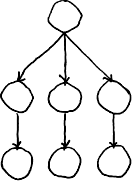
\includegraphics[width = \similaritySize]{figures/expert-52-trim.png}\end{minipage}\begin{minipage}{\similarityArrowSize}$\leftrightarrow$\end{minipage}\begin{minipage}{\similaritySize}\includegraphics[width = \similaritySize]{figures/expert-79-trim.png}\end{minipage}\\\\
%%       \begin{minipage}{\similaritySize}\includegraphics[width = \similaritySize]{figures/expert-16-trim.png}\end{minipage}\begin{minipage}{\similarityArrowSize}$\leftrightarrow$\end{minipage}\begin{minipage}{\similaritySize}\includegraphics[width = \similaritySize]{figures/expert-17-trim.png}\end{minipage}
%%     \end{tabular} &
    
%%     \begin{tabular}{l}
%%       \begin{minipage}{\similaritySize}\includegraphics[width = \similaritySize]{figures/expert-22-trim.png}\end{minipage}\begin{minipage}{\similarityArrowSize}$\leftrightarrow$\end{minipage}\begin{minipage}{\similaritySize}\includegraphics[width = \similaritySize]{figures/expert-77-trim.png}\end{minipage}\\\\
%%       \begin{minipage}{\similaritySize}\includegraphics[width = \similaritySize]{figures/expert-64-trim.png}\end{minipage}\begin{minipage}{\similarityArrowSize}$\leftrightarrow$\end{minipage}\begin{minipage}{\similaritySize}\includegraphics[width = \similaritySize]{figures/expert-97-trim.png}\end{minipage}
%%     \end{tabular}
%% \\&\\    \hline
%%     %\\
%% %    \multicolumn{1}{c|}{}&&\\\cline{2-3}
%% %    \multicolumn{1}{c|}{}&&\\ \multicolumn{1}{c|}{}
%%     %& %% \begin{tabular}{l}
%%     %%   \begin{minipage}{\similaritySize}\includegraphics[width = \similaritySize]{figures/expert-52-trim.png}\end{minipage}\begin{minipage}{\similarityArrowSize}$\leftrightarrow$\end{minipage}\begin{minipage}{\similaritySize}\includegraphics[width = \similaritySize]{figures/expert-79-trim.png}\end{minipage}\\\\
%%     %%   \begin{minipage}{\similaritySize}\includegraphics[width = \similaritySize]{figures/expert-16-trim.png}\end{minipage}\begin{minipage}{\similarityArrowSize}$\leftrightarrow$\end{minipage}\begin{minipage}{\similaritySize}\includegraphics[width = \similaritySize]{figures/expert-17-trim.png}\end{minipage}
%%     %% \end{tabular}
%%     %&
%%     %% \begin{tabular}{l}
%%     %%   \begin{minipage}{\similaritySize}\includegraphics[width = \similaritySize]{figures/expert-75-extra-trim.png}\end{minipage}\begin{minipage}{\similarityArrowSize}$\leftrightarrow$\end{minipage}\begin{minipage}{\similaritySize}\includegraphics[width = \similaritySize]{figures/expert-89-trim.png}\end{minipage}\\\\
%%     %%   \begin{minipage}{\similaritySize}\includegraphics[width = \similaritySize]{figures/expert-3-trim.png}\end{minipage}\begin{minipage}{\similarityArrowSize}$\leftrightarrow$\end{minipage}\begin{minipage}{\similaritySize}\includegraphics[width = \similaritySize]{figures/expert-39-trim.png}\end{minipage}
%%     %% \end{tabular}
%% %\\ \multicolumn{1}{c|}{}&&\\\cline{2-3}\cline{2-3}
%%   \end{tabular}
  
%%   \centering
%% \caption{Pairs of images either close together or far apart in different features spaces.  The symbol $\leftrightarrow$ points to the compared images. Features of the program capture abstract notions like symmetry and repetition. Distance metric over images is $L_{\text{learned}}(\cdot|\cdot)$ (see Sec.~\ref{generalizingTheHandDrawings}). Similarity of programs captures high-level features like repetition and symmetry, whereas similarity of images corresponds to similar drawing commands being in similar places. See Sec. 2 of the supplement for more examples.}\label{similarityMatrix}  \end{figure}

%% We project these features down to a
%% 2-dimensional subspace using primary component analysis
%% (PCA); see Fig.\ref{NMF}.  One could use many
%% alternative similarity metrics between drawings which would capture pixel-level similarities while missing high-level geometric similarities.
%% We used our learned distance metric between traces, $L_{\text{learned}}(\cdot|\cdot)$, and projected to a 2-dimensional subspace using multidimensional scaling (MDS:~\cite{cox2008multidimensional}). This reveals similarities between the objects in the drawings,
%% while missing similarities at the level of the program.
%% \begin{figure}[h]
%% \centering  \begin{minipage}{\textwidth}\centering
%%   %\includegraphics[width = 0.69\textwidth]{figures/PCA.png}
%%   \includegraphics[width = 0.69\textwidth]{figures/PCA_improved.png}
%%     \caption{PCA on features of the programs that were synthesized for each drawing. Symmetric figures cluster to the right; ``loopy'' figures cluster to the left; complicated programs are at the top and simple programs are at the bottom.}    \label{NMF}
%%   \end{minipage} %\hfill
%%   \begin{minipage}{\textwidth}\centering
%%     \includegraphics[width = 0.69\textwidth]{figures/imageSimilarity.png} 
%%     \caption{MDS on drawings using the learned distance metric, $L_{\text{learned}}(\cdot|\cdot)$. Drawings with similar looking parts in similar locations are clustered together.}
%%   \end{minipage}
%% \end{figure}

\subsection{Extrapolating figures}
Having access to the source code of a graphics program facilitates coherent, high-level image editing.
%For example,
%we could change all of the circles to squares or make all of the lines be dashed.
For example we can extrapolate figures
by increasing the number of times that loops are executed.
Extrapolating repetitive visuals patterns comes naturally to humans,
and is a practical application:
imagine hand drawing a repetitive graphical model structure
and having our system automatically induce and extend the pattern.
Fig.~\ref{extrapolationFigure} shows extrapolations produced by our system.
\begin{figure}[H]\centering
  \includegraphics[width = 0.885\textwidth]{figures/extrapolationMatrix1.png}
  \includegraphics[width = 0.885\textwidth]{figures/extrapolationMatrix2.png}
%  \includegraphics[width = \textwidth]{figures/extrapolationMatrix3.png}  
   \caption{Top, white: hand drawings. Bottom, black: extrapolations produced by our system.}
  \label{extrapolationFigure}
  \end{figure}
%
            \begin{tabular}{ll}
    \includegraphics[width = 5cm]{../TikZ/drawings/expert-17.png}&
    \includegraphics[width = 5cm]{../TikZ/extrapolations/expert-17-extrapolation.png}
    \end{tabular}        
            \\

            \begin{tabular}{ll}
    \includegraphics[width = 5cm]{../TikZ/drawings/expert-21.png}&
    \includegraphics[width = 5cm]{../TikZ/extrapolations/expert-21-extrapolation.png}
    \end{tabular}        
            \\

            \begin{tabular}{ll}
    \includegraphics[width = 5cm]{../TikZ/drawings/expert-7.png}&
    \includegraphics[width = 5cm]{../TikZ/extrapolations/expert-7-extrapolation.png}
    \end{tabular}        
            \\

            \begin{tabular}{ll}
    \includegraphics[width = 5cm]{../TikZ/drawings/expert-36.png}&
    \includegraphics[width = 5cm]{../TikZ/extrapolations/expert-36-extrapolation.png}
    \end{tabular}        
            \\

            \begin{tabular}{ll}
    \includegraphics[width = 5cm]{../TikZ/drawings/expert-58.png}&
    \includegraphics[width = 5cm]{../TikZ/extrapolations/expert-58-extrapolation.png}
    \end{tabular}        
            \\

            \begin{tabular}{ll}
    \includegraphics[width = 5cm]{../TikZ/drawings/expert-22.png}&
    \includegraphics[width = 5cm]{../TikZ/extrapolations/expert-22-extrapolation.png}
    \end{tabular}        
            \\

            \begin{tabular}{ll}
    \includegraphics[width = 5cm]{../TikZ/drawings/expert-14.png}&
    \includegraphics[width = 5cm]{../TikZ/extrapolations/expert-14-extrapolation.png}
    \end{tabular}        
            \\

            \begin{tabular}{ll}
    \includegraphics[width = 5cm]{../TikZ/drawings/expert-68.png}&
    \includegraphics[width = 5cm]{../TikZ/extrapolations/expert-68-extrapolation.png}
    \end{tabular}        
            \\

            \begin{tabular}{ll}
    \includegraphics[width = 5cm]{../TikZ/drawings/expert-12.png}&
    \includegraphics[width = 5cm]{../TikZ/extrapolations/expert-12-extrapolation.png}
    \end{tabular}        
            \\

            \begin{tabular}{ll}
    \includegraphics[width = 5cm]{../TikZ/drawings/expert-35.png}&
    \includegraphics[width = 5cm]{../TikZ/extrapolations/expert-35-extrapolation.png}
    \end{tabular}        
            \\

            \begin{tabular}{ll}
    \includegraphics[width = 5cm]{../TikZ/drawings/expert-31.png}&
    \includegraphics[width = 5cm]{../TikZ/extrapolations/expert-31-extrapolation.png}
    \end{tabular}        
            \\

            \begin{tabular}{ll}
    \includegraphics[width = 5cm]{../TikZ/drawings/expert-37.png}&
    \includegraphics[width = 5cm]{../TikZ/extrapolations/expert-37-extrapolation.png}
    \end{tabular}        
            \\

            \begin{tabular}{ll}
    \includegraphics[width = 5cm]{../TikZ/drawings/expert-29.png}&
    \includegraphics[width = 5cm]{../TikZ/extrapolations/expert-29-extrapolation.png}
    \end{tabular}        
            \\

            \begin{tabular}{ll}
    \includegraphics[width = 5cm]{../TikZ/drawings/expert-57.png}&
    \includegraphics[width = 5cm]{../TikZ/extrapolations/expert-57-extrapolation.png}
    \end{tabular}        
            \\

            \begin{tabular}{ll}
    \includegraphics[width = 5cm]{../TikZ/drawings/expert-23.png}&
    \includegraphics[width = 5cm]{../TikZ/extrapolations/expert-23-extrapolation.png}
    \end{tabular}        
            \\

            \begin{tabular}{ll}
    \includegraphics[width = 5cm]{../TikZ/drawings/expert-60.png}&
    \includegraphics[width = 5cm]{../TikZ/extrapolations/expert-60-extrapolation.png}
    \end{tabular}        
            \\

            \begin{tabular}{ll}
    \includegraphics[width = 5cm]{../TikZ/drawings/expert-16.png}&
    \includegraphics[width = 5cm]{../TikZ/extrapolations/expert-16-extrapolation.png}
    \end{tabular}        
            \\

            \begin{tabular}{ll}
    \includegraphics[width = 5cm]{../TikZ/drawings/expert-5.png}&
    \includegraphics[width = 5cm]{../TikZ/extrapolations/expert-5-extrapolation.png}
    \end{tabular}        
            \\

            \begin{tabular}{ll}
    \includegraphics[width = 5cm]{../TikZ/drawings/expert-50.png}&
    \includegraphics[width = 5cm]{../TikZ/extrapolations/expert-50-extrapolation.png}
    \end{tabular}        
            \\

            \begin{tabular}{ll}
    \includegraphics[width = 5cm]{../TikZ/drawings/expert-6.png}&
    \includegraphics[width = 5cm]{../TikZ/extrapolations/expert-6-extrapolation.png}
    \end{tabular}        
            



% \remark{Seems like you're still fleshing this part out, but I'll give my feedback anyway: (1) This subsection could really use a motivational introduction, e.g. ``The program synthesizer can help correct errors/bad proposals from the neural network by favoring execution traces which lead to more concise/general programs.'' (2) The image likelihood function should probably be introduced sooner, when you talk about SMC/beam search. (3) Where does $\theta$ come from? Is it set by hand? Learned? (4) How does Eq. 4 get used? Is this a modification to the beam search objective / SMC posterior? If so, it'd be great to have set up the version without it in an earlier section, and then be able to refer to this as a small modification of the previous equation.}


%\pagebreak
%\section{Discussion}

\section{Related work}

\textbf{Program Induction:}
Our approach to learning to search for programs draws theoretical
underpinnings from Levin
search~\citep{levin1973universal,solomonoff1984optimum} and
Schmidhuber's OOPS model~\citep{schmidhuber2004optimal}.
DeepCoder~\citep{BalGauBroetal16} is a recent model which, like ours, learns to predict likely program components.
Our work differs because we treat
the problem as \emph{metareasoning}, identifying and modeling
the trade-off between tractability and probability of success.
TerpreT~\citep{gaunt2016terpret} 
systematically compares constraint-based program synthesis techniques
against gradient-based search techniques, like those used to train
Differentiable Neural Computers~\citep{graves2016hybrid}.  The TerpreT
experiments motivate our use of constraint-based techniques.



\textbf{Deep Learning:} Our neural network bears resemblance to the Attend-Infer-Repeat (AIR) system, which learns to decompose an image into its constituent objects~\citep{eslami1603attend}. AIR learns an iterative inference scheme which infers objects one by one and also decides when to stop inference.
%; this is similar to our approach's first stage, which parses images into traces. Our approach further produces interpretable, symbolic programs which generate those traces.
Our network  differs in its architecture and training regime: AIR learns a recurrent auto-encoding model via variational inference, whereas our parsing stage learns an autoregressive-style model from randomly-generated (trace, image) pairs.
%Finally, while AIR was evaluated on multi-MNIST images and synthetic 3D scenes, we focus on hand-drawn sketches.

IM2LATEX~\citep{im2latex} is a recent work that also converts images to
~\LaTeX.
Their goal is to derender  \LaTeX~ equations,
which recovers a markup language representation.
Our goal is to go from
noisy input to a high-level program,
which goes beyond markup languages by supporting
programming constructs like loops and conditionals.
Recovering a high-level program is more challenging than recovering markup
because it is a highly under constrained symbolic reasoning problem.


Our image-to-trace parsing architecture builds on prior work on controlling procedural graphics programs~\citep{ritchie2016neurally}.
%Given a program which generates random 2D recursive structures such as vines, that system learns a structurally-identical ``guide program'' whose output can be directed, via neural networks, to resemble a given target image. 
We adapt this method to a different visual domain (figures composed of multiple objects), using a broad prior over possible scenes as the initial program and viewing the trace through the guide program as a symbolic parse of the target image.
We then show how to efficiently synthesize higher-level programs from these traces.

In the computer graphics literature, there have been other systems which convert sketches into procedural representations. One uses a convolutional network to match a sketch to the output of a parametric 3D modeling system~\citep{huang2017shape}. Another uses convolutional networks to support sketch-based instantiation of procedural primitives within an interactive architectural modeling system~\citep{Nishida:2016:ISU:2897824.2925951}. Both systems focus on inferring fixed-dimensional parameter vectors. In contrast, we seek to automatically infer a structured, programmatic representation of a sketch which captures higher-level visual patterns.

\textbf{Hand-drawn sketches:} Prior work has also applied sketch-based program synthesis to authoring graphics programs. Sketch-n-Sketch is a bi-directional editing system in which direct manipulations to a program's output automatically propagate to the program source code~\citep{Hempel:2016:SSP:2984511.2984575}. We see this work as complementary to our own: programs produced by our method could be provided to a Sketch-n-Sketch-like system as a starting point for further editing.

The CogSketch system~\citep{forbus2011cogsketch} also aims to have a high-level understanding of hand-drawn figures. Their primary goal is cognitive modeling (they apply their system to solving IQ-test style visual reasoning problems), whereas we are interested in building an automated AI application (e.g. in our system the user need not annotate which strokes correspond to which shapes; our neural network produces something equivalent to the annotations).
%A key similarity however is that both CogSketch and our system have as a goal to make it easier to produce nice-looking figures.
%% Unsupervised Program Synthesis~\cite{ellis2015unsupervised} is a related framework which was also applied to geometric reasoning problems. The goals of~\cite{ellis2015unsupervised} were cognitive modeling,
%% and they applied their technique to synthetic scenes used in human behavioral studies.
%% open domain sketch understanding. structure mapping style model. also taps into cyc? the user segments the ink and labels them with concepts from knowledge base. like us they focus on compositional understanding. ``cognitive simulation", solves things like Raven matrices in IQ tests. not really trying right now to be automated like our system.

\textbf{The Trace Hypothesis:} The idea that an execution trace could assist in program learning goes back to the 1970's~\citep{Summers:1977:MLP:321992.322002} and has  been applied in neural models of program induction, like Neural Program Interpreters~\citep{DBLP:journals/corr/ReedF15}, or DeepCoder, which predicts what functions occur in the execution trace~\citep{BalGauBroetal16}.
Our contribution to this idea is the trace hypothesis:
that  trace sets can be inferred from perceptual data,
and that the trace set is a useful bridge between perception and symbolic representation.
Our work is the first to articulate and explore this hypothesis
by demonstrating how a trace could be inferred and how it can be used to synthesize a high-level program.


%% \subsection{Future work}
%% There are many directions for future work. The proposal network  currently handles only a very small subset of \LaTeX~drawing commands, though there is no reason that it could not be extended to handle more with a higher-capacity network.
%% In the synthesis phase, a more expressive DSL---including subroutines, recursion, and symmetry groups beyond reflections---would allow the system to effectively model a wider variety of graphical phenomena. The synthesizer itself could also be the subject of future work: the system currently uses the general-purpose Sketch synthesizer, which can take minutes to hours to run, whereas custom-built domain-specific synthesizers can run much faster or even interactively~\citep{le2014flashextract}.

%% In the parsing phase, the proposal network currently samples positional variables on a discrete grid. More general types of drawings could be supported by instead sampling from continuous distributions, e.g. using Mixture Density Networks (MDN)~\citep{MDN}.
%% We prototyped a variant of our model that predicts continuous coordinates. See supplement.

\section{Contributions}

We have presented a system for inferring graphics programs which generate \LaTeX-style figures from hand-drawn images. The system uses a combination of deep neural networks and stochastic search to parse drawings into symbolic trace sets; it then feeds these traces to a general-purpose program synthesis engine to infer a structured graphics program. We evaluated our model's performance at parsing novel images, and we demonstrated its ability to extrapolate from provided drawings.


In the near future, we believe it will be possible to produce professional-looking figures just by drawing them and then letting an artificially-intelligent agent write the code.
More generally, we believe the trace hypothesis, as realized in our two-phase system---parsing into trace sets, then searching for a low-cost symbolic program which generates those traces---may be a useful paradigm for other domains in which agents must programmatically reason about noisy perceptual input.


%% \subsubsection*{Acknowledgments} We are grateful for advice from Will Grathwohl and Jiajun Wu on the design of the neural architecture.

%% \subsubsection*{Supplemental information.} The supplement may be found at:~\url{http://web.mit.edu/ellisk/www/graphicsProgramSupplement.pdf}


%
            \begin{tabular}{lll}
    \includegraphics[width = 5cm]{../TikZ/drawings/expert-0.png}&
            \includegraphics[width = 5cm]{../TikZ/drawings/expert-0-parses/0.png}&
    
        \begin{minipage}{10cm}
        \begin{verbatim}
line(6,2,6,3,
arrow = False,solid = True);
line(6,2,3,2,
arrow = True,solid = True);
reflect(reflect(y = 9)){
line(3,2,5,4,
arrow = True,solid = True);
rectangle(0,0,8,9);
rectangle(5,3,7,6);
rectangle(1,1,3,3)
}
        \end{verbatim}
\end{minipage}

    \end{tabular}        
            \\

            \begin{tabular}{lll}
    \includegraphics[width = 5cm]{../TikZ/drawings/expert-1.png}&
            \includegraphics[width = 5cm]{../TikZ/drawings/expert-1-parses/0.png}&
    
        \begin{minipage}{10cm}
        \begin{verbatim}
Solver timeout
        \end{verbatim}
\end{minipage}

    \end{tabular}        
            \\

            \begin{tabular}{lll}
    \includegraphics[width = 5cm]{../TikZ/drawings/expert-2.png}&
            \includegraphics[width = 5cm]{../TikZ/drawings/expert-2-parses/0.png}&
    
        \begin{minipage}{10cm}
        \begin{verbatim}
rectangle(4,2,6,5);
reflect(reflect(y = 7)){
line(2,6,4,4,
arrow = True,solid = True);
rectangle(0,0,2,2)
}
        \end{verbatim}
\end{minipage}

    \end{tabular}        
            \\

            \begin{tabular}{lll}
    \includegraphics[width = 5cm]{../TikZ/drawings/expert-3.png}&
            \includegraphics[width = 5cm]{../TikZ/drawings/expert-3-parses/0.png}&
    
        \begin{minipage}{10cm}
        \begin{verbatim}
circle(10,5);
line(7,5,9,5,
arrow = True,solid = True);
rectangle(5,3,7,7);
rectangle(0,0,12,10);
reflect(reflect(y = 10)){
line(3,8,5,6,
arrow = True,solid = True);
rectangle(1,7,3,9)
}
        \end{verbatim}
\end{minipage}

    \end{tabular}        
            \\

            \begin{tabular}{lll}
    \includegraphics[width = 5cm]{../TikZ/drawings/expert-4.png}&
            \includegraphics[width = 5cm]{../TikZ/drawings/expert-4-parses/0.png}&
    
        \begin{minipage}{10cm}
        \begin{verbatim}
circle(10,4);
line(10,1,2,1,
arrow = True,solid = False);
line(10,1,10,3,
arrow = False,solid = False);
line(7,4,9,4,
arrow = True,solid = True);
reflect(reflect(y = 8)){
line(2,7,4,5,
arrow = True,solid = True);
rectangle(4,2,7,6);
rectangle(0,6,2,8)
}
        \end{verbatim}
\end{minipage}

    \end{tabular}        
            \\

            \begin{tabular}{lll}
    \includegraphics[width = 5cm]{../TikZ/drawings/expert-5.png}&
            \includegraphics[width = 5cm]{../TikZ/drawings/expert-5-parses/0.png}&
    
        \begin{minipage}{10cm}
        \begin{verbatim}
Solver timeout
        \end{verbatim}
\end{minipage}

    \end{tabular}        
            \\

            \begin{tabular}{lll}
    \includegraphics[width = 5cm]{../TikZ/drawings/expert-6.png}&
            \includegraphics[width = 5cm]{../TikZ/drawings/expert-6-parses/0.png}&
    
        \begin{minipage}{10cm}
        \begin{verbatim}
line(0,1,2,0,
arrow = False,solid = True);
for (i < 3){
if (i > 0){
line(3*i + -3,4,3*i + -1,3,
arrow = False,solid = True);
line(0,3*i + -2,3*i + -3,4,
arrow = False,solid = True)
}
rectangle(2,0,5,3)
}
        \end{verbatim}
\end{minipage}

    \end{tabular}        
            \\

            \begin{tabular}{lll}
    \includegraphics[width = 5cm]{../TikZ/drawings/expert-7.png}&
            \includegraphics[width = 5cm]{../TikZ/drawings/expert-7-parses/0.png}&
    
        \begin{minipage}{10cm}
        \begin{verbatim}
for (i < 3){
circle(-3*i + 7,1);
circle(-3*i + 7,6);
line(-3*i + 7,-1*i + 4,-3*i + 7,5,
arrow = False,solid = True)
}
        \end{verbatim}
\end{minipage}

    \end{tabular}        
            \\

            \begin{tabular}{lll}
    \includegraphics[width = 5cm]{../TikZ/drawings/expert-8.png}&
            \includegraphics[width = 5cm]{../TikZ/drawings/expert-8-parses/0.png}&
    
        \begin{minipage}{10cm}
        \begin{verbatim}
line(0,0,0,4,
arrow = False,solid = True)
        \end{verbatim}
\end{minipage}

    \end{tabular}        
            \\

            \begin{tabular}{lll}
    \includegraphics[width = 5cm]{../TikZ/drawings/expert-9.png}&
            \includegraphics[width = 5cm]{../TikZ/drawings/expert-9-parses/0.png}&
    
        \begin{minipage}{10cm}
        \begin{verbatim}
line(6,0,0,0,
arrow = True,solid = True)
        \end{verbatim}
\end{minipage}

    \end{tabular}        
            \\

            \begin{tabular}{lll}
    \includegraphics[width = 5cm]{../TikZ/drawings/expert-10.png}&
            \includegraphics[width = 5cm]{../TikZ/drawings/expert-10-parses/0.png}&
    
        \begin{minipage}{10cm}
        \begin{verbatim}
rectangle(0,0,3,4)
        \end{verbatim}
\end{minipage}

    \end{tabular}        
            \\

            \begin{tabular}{lll}
    \includegraphics[width = 5cm]{../TikZ/drawings/expert-11.png}&
            \includegraphics[width = 5cm]{../TikZ/drawings/expert-11-parses/0.png}&
    
        \begin{minipage}{10cm}
        \begin{verbatim}
circle(1,1)
        \end{verbatim}
\end{minipage}

    \end{tabular}        
            \\

            \begin{tabular}{lll}
    \includegraphics[width = 5cm]{../TikZ/drawings/expert-12.png}&
            \includegraphics[width = 5cm]{../TikZ/drawings/expert-12-parses/0.png}&
    
        \begin{minipage}{10cm}
        \begin{verbatim}
line(2,6,5,6,
arrow = False,solid = True);
reflect(reflect(x = 7)){
circle(6,1);
line(2,1,5,1,
arrow = False,solid = True);
line(1,2,1,5,
arrow = False,solid = True);
rectangle(5,5,7,7)
}
        \end{verbatim}
\end{minipage}

    \end{tabular}        
            \\

            \begin{tabular}{lll}
    \includegraphics[width = 5cm]{../TikZ/drawings/expert-13.png}&
            \includegraphics[width = 5cm]{../TikZ/drawings/expert-13-parses/0.png}&
    
        \begin{minipage}{10cm}
        \begin{verbatim}
line(2,1,4,1,
arrow = True,solid = True);
line(3,2,1,2,
arrow = True,solid = True);
line(5,0,3,0,
arrow = True,solid = True);
line(0,3,2,3,
arrow = True,solid = True)
        \end{verbatim}
\end{minipage}

    \end{tabular}        
            \\

            \begin{tabular}{lll}
    \includegraphics[width = 5cm]{../TikZ/drawings/expert-14.png}&
            \includegraphics[width = 5cm]{../TikZ/drawings/expert-14-parses/0.png}&
    
        \begin{minipage}{10cm}
        \begin{verbatim}
for (i < 4){
if (i > 0){
rectangle(-2*i + 6,2*i + -2,-2*i + 7,2*i + -1)
}
rectangle(-2*i + 6,2*i,-2*i + 7,2*i + 1)
}
        \end{verbatim}
\end{minipage}

    \end{tabular}        
            \\

            \begin{tabular}{lll}
    \includegraphics[width = 5cm]{../TikZ/drawings/expert-15.png}&
            \includegraphics[width = 5cm]{../TikZ/drawings/expert-15-parses/0.png}&
    
        \begin{minipage}{10cm}
        \begin{verbatim}
line(0,3,2,3,
arrow = False,solid = False);
line(2,1,4,1,
arrow = False,solid = False);
line(1,2,3,2,
arrow = False,solid = True);
line(3,0,5,0,
arrow = False,solid = True)
        \end{verbatim}
\end{minipage}

    \end{tabular}        
            \\

            \begin{tabular}{lll}
    \includegraphics[width = 5cm]{../TikZ/drawings/expert-16.png}&
            \includegraphics[width = 5cm]{../TikZ/drawings/expert-16-parses/0.png}&
    
        \begin{minipage}{10cm}
        \begin{verbatim}
for (i < 4){
if (i > 0){
circle(-2*i + 7,3*i + -2);
line(-2*i + 9,3*i,-2*i + 10,3*i + -2,
arrow = False,solid = True);
line(-2*i + 8,3*i + -2,-2*i + 9,3*i,
arrow = False,solid = True)
}
circle(-2*i + 9,3*i + 1)
}
        \end{verbatim}
\end{minipage}

    \end{tabular}        
            \\

            \begin{tabular}{lll}
    \includegraphics[width = 5cm]{../TikZ/drawings/expert-17.png}&
            \includegraphics[width = 5cm]{../TikZ/drawings/expert-17-parses/0.png}&
    
        \begin{minipage}{10cm}
        \begin{verbatim}
for (i < 4){
if (i > 0){
line(2*i + 1,-3*i + 12,2*i,-3*i + 10,
arrow = True,solid = True);
line(2*i + 1,-3*i + 12,2*i + 2,-3*i + 10,
arrow = True,solid = True);
rectangle(2*i + -2,-3*i + 9,2*i,-3*i + 11)
}
rectangle(2*i + 2,-3*i + 9,2*i + 4,-3*i + 11)
}
        \end{verbatim}
\end{minipage}

    \end{tabular}        
            \\

            \begin{tabular}{lll}
    \includegraphics[width = 5cm]{../TikZ/drawings/expert-18.png}&
            \includegraphics[width = 5cm]{../TikZ/drawings/expert-18-parses/0.png}&
    
        \begin{minipage}{10cm}
        \begin{verbatim}
circle(5,1);
for (i < 3){
if (i > 0){
circle(7,2*i + -1);
circle(i + 2,2*i + 1)
}
circle(1,6)
}
        \end{verbatim}
\end{minipage}

    \end{tabular}        
            \\

            \begin{tabular}{lll}
    \includegraphics[width = 5cm]{../TikZ/drawings/expert-19.png}&
            \includegraphics[width = 5cm]{../TikZ/drawings/expert-19-parses/0.png}&
    
        \begin{minipage}{10cm}
        \begin{verbatim}
line(4,4,2,2,
arrow = True,solid = True);
rectangle(3,4,5,6);
rectangle(0,0,2,2)
        \end{verbatim}
\end{minipage}

    \end{tabular}        
            \\

            \begin{tabular}{lll}
    \includegraphics[width = 5cm]{../TikZ/drawings/expert-20.png}&
            \includegraphics[width = 5cm]{../TikZ/drawings/expert-20-parses/0.png}&
    
        \begin{minipage}{10cm}
        \begin{verbatim}
rectangle(0,4,2,6);
for (i < 3){
if (i > 0){
line(-4*i + 12,5,-4*i + 10,5,
arrow = True,solid = True);
for (j < i + 1){
circle(-4*j + 9,-4*i + 9)
}
}
line(-4*i + 9,4,-4*i + 9,2,
arrow = True,solid = True)
}
        \end{verbatim}
\end{minipage}

    \end{tabular}        
            \\

            \begin{tabular}{lll}
    \includegraphics[width = 5cm]{../TikZ/drawings/expert-21.png}&
            \includegraphics[width = 5cm]{../TikZ/drawings/expert-21-parses/0.png}&
    
        \begin{minipage}{10cm}
        \begin{verbatim}
Solver timeout
        \end{verbatim}
\end{minipage}

    \end{tabular}        
            \\

            \begin{tabular}{lll}
    \includegraphics[width = 5cm]{../TikZ/drawings/expert-22.png}&
            \includegraphics[width = 5cm]{../TikZ/drawings/expert-22-parses/0.png}&
    
        \begin{minipage}{10cm}
        \begin{verbatim}
for (i < 3){
line(-4*i + 9,4,-4*i + 9,2,
arrow = True,solid = True);
for (j < 2){
line(-4*j + 8,5,-4*j + 6,5,
arrow = True,solid = True);
rectangle(-4*i + 8,4*j,-4*i + 10,4*j + 2)
}
}
        \end{verbatim}
\end{minipage}

    \end{tabular}        
            \\

            \begin{tabular}{lll}
    \includegraphics[width = 5cm]{../TikZ/drawings/expert-23.png}&
            \includegraphics[width = 5cm]{../TikZ/drawings/expert-23-parses/0.png}&
    
        \begin{minipage}{10cm}
        \begin{verbatim}
for (i < 3){
if (i > 0){
line(-4*i + 12,1,-4*i + 10,1,
arrow = True,solid = True)
}
circle(-4*i + 9,1);
circle(-4*i + 9,5);
line(-4*i + 9,2,-4*i + 9,4,
arrow = True,solid = True)
}
        \end{verbatim}
\end{minipage}

    \end{tabular}        
            \\

            \begin{tabular}{lll}
    \includegraphics[width = 5cm]{../TikZ/drawings/expert-24.png}&
            \includegraphics[width = 5cm]{../TikZ/drawings/expert-24-parses/0.png}&
    
        \begin{minipage}{10cm}
        \begin{verbatim}
reflect(reflect(x = 6)){
for (i < 3){
if (i > 0){
line(-2*i + 7,-4*i + 11,-2*i + 7,-4*i + 10,
arrow = True,solid = True);
rectangle(0,-4*i + 11,6,-3*i + 12)
}
rectangle(2,0,4,2)
}
}
        \end{verbatim}
\end{minipage}

    \end{tabular}        
            \\

            \begin{tabular}{lll}
    \includegraphics[width = 5cm]{../TikZ/drawings/expert-25.png}&
            \includegraphics[width = 5cm]{../TikZ/drawings/expert-25-parses/0.png}&
    
        \begin{minipage}{10cm}
        \begin{verbatim}
for (i < 3){
if (i > 0){
line(3*i,1,3*i + -1,1,
arrow = True,solid = True)
}
rectangle(3*i,0,3*i + 2,2)
}
        \end{verbatim}
\end{minipage}

    \end{tabular}        
            \\

            \begin{tabular}{lll}
    \includegraphics[width = 5cm]{../TikZ/drawings/expert-26.png}&
            \includegraphics[width = 5cm]{../TikZ/drawings/expert-26-parses/0.png}&
    
        \begin{minipage}{10cm}
        \begin{verbatim}
line(1,3,1,4,
arrow = False,solid = True);
for (i < 3){
if (i > 0){
line(1,-5*i + 13,1,-4*i + 10,
arrow = True,solid = True)
}
circle(1,-4*i + 9)
}
        \end{verbatim}
\end{minipage}

    \end{tabular}        
            \\

            \begin{tabular}{lll}
    \includegraphics[width = 5cm]{../TikZ/drawings/expert-27.png}&
            \includegraphics[width = 5cm]{../TikZ/drawings/expert-27-parses/0.png}&
    
        \begin{minipage}{10cm}
        \begin{verbatim}
reflect(reflect(x = 2)){
line(0,1,1,2,
arrow = False,solid = True);
line(1,0,2,1,
arrow = False,solid = True)
}
        \end{verbatim}
\end{minipage}

    \end{tabular}        
            \\

            \begin{tabular}{lll}
    \includegraphics[width = 5cm]{../TikZ/drawings/expert-28.png}&
            \includegraphics[width = 5cm]{../TikZ/drawings/expert-28-parses/0.png}&
    
        \begin{minipage}{10cm}
        \begin{verbatim}
line(0,0,0,2,
arrow = False,solid = True);
line(0,2,2,2,
arrow = False,solid = True)
        \end{verbatim}
\end{minipage}

    \end{tabular}        
            \\

            \begin{tabular}{lll}
    \includegraphics[width = 5cm]{../TikZ/drawings/expert-29.png}&
            \includegraphics[width = 5cm]{../TikZ/drawings/expert-29-parses/0.png}&
    
        \begin{minipage}{10cm}
        \begin{verbatim}
for (i < 3){
line(i,-1*i + 6,2*i + 2,-1*i + 6,
arrow = False,solid = True);
line(i,-2*i + 4,i,-1*i + 6,
arrow = False,solid = True)
}
        \end{verbatim}
\end{minipage}

    \end{tabular}        
            \\

            \begin{tabular}{lll}
    \includegraphics[width = 5cm]{../TikZ/drawings/expert-30.png}&
            \includegraphics[width = 5cm]{../TikZ/drawings/expert-30-parses/0.png}&
    
        \begin{minipage}{10cm}
        \begin{verbatim}
for (i < 3){
if (i > 0){
circle(1,-3*i + 7);
circle(5,-2*i + 6);
rectangle(0,-3*i + 6,2,-3*i + 8)
}
rectangle(4,1,6,5)
}
        \end{verbatim}
\end{minipage}

    \end{tabular}        
            \\

            \begin{tabular}{lll}
    \includegraphics[width = 5cm]{../TikZ/drawings/expert-31.png}&
            \includegraphics[width = 5cm]{../TikZ/drawings/expert-31-parses/0.png}&
    
        \begin{minipage}{10cm}
        \begin{verbatim}
for (i < 3){
rectangle(3*i,-2*i + 4,3*i + 2,6);
for (j < i + 1){
circle(3*i + 1,-2*j + 5)
}
}
        \end{verbatim}
\end{minipage}

    \end{tabular}        
            \\

            \begin{tabular}{lll}
    \includegraphics[width = 5cm]{../TikZ/drawings/expert-32.png}&
            \includegraphics[width = 5cm]{../TikZ/drawings/expert-32-parses/0.png}&
    
        \begin{minipage}{10cm}
        \begin{verbatim}
circle(5,5);
line(2,5,4,5,
arrow = False,solid = True);
rectangle(0,0,5,3);
rectangle(0,4,2,6)
        \end{verbatim}
\end{minipage}

    \end{tabular}        
            \\

            \begin{tabular}{lll}
    \includegraphics[width = 5cm]{../TikZ/drawings/expert-33.png}&
            \includegraphics[width = 5cm]{../TikZ/drawings/expert-33-parses/0.png}&
    
        \begin{minipage}{10cm}
        \begin{verbatim}
line(0,0,6,0,
arrow = False,solid = False);
reflect(reflect(x = 6)){
line(6,0,6,3,
arrow = False,solid = True);
line(0,3,6,3,
arrow = False,solid = False)
}
        \end{verbatim}
\end{minipage}

    \end{tabular}        
            \\

            \begin{tabular}{lll}
    \includegraphics[width = 5cm]{../TikZ/drawings/expert-34.png}&
            \includegraphics[width = 5cm]{../TikZ/drawings/expert-34-parses/0.png}&
    
        \begin{minipage}{10cm}
        \begin{verbatim}
Solver timeout
        \end{verbatim}
\end{minipage}

    \end{tabular}        
            \\

            \begin{tabular}{lll}
    \includegraphics[width = 5cm]{../TikZ/drawings/expert-35.png}&
            \includegraphics[width = 5cm]{../TikZ/drawings/expert-35-parses/0.png}&
    
        \begin{minipage}{10cm}
        \begin{verbatim}
for (i < 3){
if (i > 0){
circle(-5*i + 11,1);
line(-1*i + 3,-1*i + 7,-5*i + 11,2,
arrow = True,solid = True)
}
circle(1,6)
}
        \end{verbatim}
\end{minipage}

    \end{tabular}        
            \\

            \begin{tabular}{lll}
    \includegraphics[width = 5cm]{../TikZ/drawings/expert-36.png}&
            \includegraphics[width = 5cm]{../TikZ/drawings/expert-36-parses/0.png}&
    
        \begin{minipage}{10cm}
        \begin{verbatim}
Solver timeout
        \end{verbatim}
\end{minipage}

    \end{tabular}        
            \\

            \begin{tabular}{lll}
    \includegraphics[width = 5cm]{../TikZ/drawings/expert-37.png}&
            \includegraphics[width = 5cm]{../TikZ/drawings/expert-37-parses/0.png}&
    
        \begin{minipage}{10cm}
        \begin{verbatim}
for (i < 3){
if (i > 0){
line(4*i + -3,-5*i + 12,2*i + 1,5,
arrow = False,solid = True);
rectangle(4*i + -4,-5*i + 10,6,-7*i + 16)
}
circle(1,8)
}
        \end{verbatim}
\end{minipage}

    \end{tabular}        
            \\

            \begin{tabular}{lll}
    \includegraphics[width = 5cm]{../TikZ/drawings/expert-38.png}&
            \includegraphics[width = 5cm]{../TikZ/drawings/expert-38-parses/0.png}&
    
        \begin{minipage}{10cm}
        \begin{verbatim}
Solver timeout
        \end{verbatim}
\end{minipage}

    \end{tabular}        
            \\

            \begin{tabular}{lll}
    \includegraphics[width = 5cm]{../TikZ/drawings/expert-39.png}&
            \includegraphics[width = 5cm]{../TikZ/drawings/expert-39-parses/0.png}&
    
        \begin{minipage}{10cm}
        \begin{verbatim}
Solver timeout
        \end{verbatim}
\end{minipage}

    \end{tabular}        
            \\

            \begin{tabular}{lll}
    \includegraphics[width = 5cm]{../TikZ/drawings/expert-40.png}&
            \includegraphics[width = 5cm]{../TikZ/drawings/expert-40-parses/0.png}&
    
        \begin{minipage}{10cm}
        \begin{verbatim}
for (i < 3){
circle(-3*i + 7,1)
}
        \end{verbatim}
\end{minipage}

    \end{tabular}        
            \\

            \begin{tabular}{lll}
    \includegraphics[width = 5cm]{../TikZ/drawings/expert-41.png}&
            \includegraphics[width = 5cm]{../TikZ/drawings/expert-41-parses/0.png}&
    
        \begin{minipage}{10cm}
        \begin{verbatim}
for (i < 3){
rectangle(-2*i + 4,0,-2*i + 5,6)
}
        \end{verbatim}
\end{minipage}

    \end{tabular}        
            \\

            \begin{tabular}{lll}
    \includegraphics[width = 5cm]{../TikZ/drawings/expert-42.png}&
            \includegraphics[width = 5cm]{../TikZ/drawings/expert-42-parses/0.png}&
    
        \begin{minipage}{10cm}
        \begin{verbatim}
line(4,0,4,1,
arrow = False,solid = False);
line(0,0,0,5,
arrow = False,solid = False);
line(4,1,4,5,
arrow = False,solid = False)
        \end{verbatim}
\end{minipage}

    \end{tabular}        
            \\

            \begin{tabular}{lll}
    \includegraphics[width = 5cm]{../TikZ/drawings/expert-43.png}&
            \includegraphics[width = 5cm]{../TikZ/drawings/expert-43-parses/0.png}&
    
        \begin{minipage}{10cm}
        \begin{verbatim}
line(4,0,4,5,
arrow = False,solid = True);
line(0,0,0,5,
arrow = False,solid = True)
        \end{verbatim}
\end{minipage}

    \end{tabular}        
            \\

            \begin{tabular}{lll}
    \includegraphics[width = 5cm]{../TikZ/drawings/expert-44.png}&
            \includegraphics[width = 5cm]{../TikZ/drawings/expert-44-parses/0.png}&
    
        \begin{minipage}{10cm}
        \begin{verbatim}
reflect(reflect(x = 12)){
circle(4,1);
line(9,1,10,1,
arrow = False,solid = True);
rectangle(0,0,2,2)
}
        \end{verbatim}
\end{minipage}

    \end{tabular}        
            \\

            \begin{tabular}{lll}
    \includegraphics[width = 5cm]{../TikZ/drawings/expert-45.png}&
            \includegraphics[width = 5cm]{../TikZ/drawings/expert-45-parses/0.png}&
    
        \begin{minipage}{10cm}
        \begin{verbatim}
rectangle(0,4,4,8);
reflect(reflect(y = 12)){
circle(7,6);
line(2,2,2,4,
arrow = True,solid = True);
line(4,6,6,6,
arrow = True,solid = True);
rectangle(1,10,3,12)
}
        \end{verbatim}
\end{minipage}

    \end{tabular}        
            \\

            \begin{tabular}{lll}
    \includegraphics[width = 5cm]{../TikZ/drawings/expert-46.png}&
            \includegraphics[width = 5cm]{../TikZ/drawings/expert-46-parses/0.png}&
    
        \begin{minipage}{10cm}
        \begin{verbatim}
reflect(reflect(y = 9)){
line(3,8,6,8,
arrow = False,solid = True);
reflect(reflect(x = 9)){
circle(1,8);
line(1,3,1,6,
arrow = False,solid = True)
}
}
        \end{verbatim}
\end{minipage}

    \end{tabular}        
            \\

            \begin{tabular}{lll}
    \includegraphics[width = 5cm]{../TikZ/drawings/expert-47.png}&
            \includegraphics[width = 5cm]{../TikZ/drawings/expert-47-parses/0.png}&
    
        \begin{minipage}{10cm}
        \begin{verbatim}
reflect(reflect(y = 11)){
rectangle(4,9,7,10);
reflect(reflect(x = 11)){
rectangle(1,4,2,7);
rectangle(8,8,11,11)
}
}
        \end{verbatim}
\end{minipage}

    \end{tabular}        
            \\

            \begin{tabular}{lll}
    \includegraphics[width = 5cm]{../TikZ/drawings/expert-48.png}&
            \includegraphics[width = 5cm]{../TikZ/drawings/expert-48-parses/0.png}&
    
        \begin{minipage}{10cm}
        \begin{verbatim}
for (i < 4){
line(i,-1*i + 5,i + 2,-1*i + 5,
arrow = False,solid = True);
line(i + 2,-1*i + 3,i + 4,-1*i + 3,
arrow = False,solid = True)
}
        \end{verbatim}
\end{minipage}

    \end{tabular}        
            \\

            \begin{tabular}{lll}
    \includegraphics[width = 5cm]{../TikZ/drawings/expert-49.png}&
            \includegraphics[width = 5cm]{../TikZ/drawings/expert-49-parses/0.png}&
    
        \begin{minipage}{10cm}
        \begin{verbatim}
for (i < 3){
if (i > 0){
rectangle(3*i + 1,-1*i + 2,3*i + 3,2);
rectangle(0,7*i + -7,3,7*i + -4)
}
rectangle(1,4,2,6)
}
        \end{verbatim}
\end{minipage}

    \end{tabular}        
            \\

            \begin{tabular}{lll}
    \includegraphics[width = 5cm]{../TikZ/drawings/expert-50.png}&
            \includegraphics[width = 5cm]{../TikZ/drawings/expert-50-parses/0.png}&
    
        \begin{minipage}{10cm}
        \begin{verbatim}
Solver timeout
        \end{verbatim}
\end{minipage}

    \end{tabular}        
            \\

            \begin{tabular}{lll}
    \includegraphics[width = 5cm]{../TikZ/drawings/expert-51.png}&
            \includegraphics[width = 5cm]{../TikZ/drawings/expert-51-parses/0.png}&
    
        \begin{minipage}{10cm}
        \begin{verbatim}
for (i < 3){
rectangle(-2*i + 4,-2*i + 4,-2*i + 7,-2*i + 5)
}
        \end{verbatim}
\end{minipage}

    \end{tabular}        
            \\

            \begin{tabular}{lll}
    \includegraphics[width = 5cm]{../TikZ/drawings/expert-52.png}&
            \includegraphics[width = 5cm]{../TikZ/drawings/expert-52-parses/0.png}&
    
        \begin{minipage}{10cm}
        \begin{verbatim}
circle(4,10);
for (i < 3){
circle(-3*i + 7,5);
circle(-3*i + 7,1);
line(-3*i + 7,4,-3*i + 7,2,
arrow = True,solid = True);
line(4,9,-3*i + 7,6,
arrow = True,solid = True)
}
        \end{verbatim}
\end{minipage}

    \end{tabular}        
            \\

            \begin{tabular}{lll}
    \includegraphics[width = 5cm]{../TikZ/drawings/expert-53.png}&
            \includegraphics[width = 5cm]{../TikZ/drawings/expert-53-parses/0.png}&
    
        \begin{minipage}{10cm}
        \begin{verbatim}
line(2,8,2,6,
arrow = True,solid = True);
line(6,8,6,4,
arrow = True,solid = True);
line(4,8,4,0,
arrow = True,solid = True);
line(0,8,8,8,
arrow = False,solid = True)
        \end{verbatim}
\end{minipage}

    \end{tabular}        
            \\

            \begin{tabular}{lll}
    \includegraphics[width = 5cm]{../TikZ/drawings/expert-54.png}&
            \includegraphics[width = 5cm]{../TikZ/drawings/expert-54-parses/0.png}&
    
        \begin{minipage}{10cm}
        \begin{verbatim}
line(2,3,2,5,
arrow = False,solid = True);
rectangle(1,1,3,3);
rectangle(1,5,3,7);
rectangle(0,0,4,8)
        \end{verbatim}
\end{minipage}

    \end{tabular}        
            \\

            \begin{tabular}{lll}
    \includegraphics[width = 5cm]{../TikZ/drawings/expert-55.png}&
            \includegraphics[width = 5cm]{../TikZ/drawings/expert-55-parses/0.png}&
    
        \begin{minipage}{10cm}
        \begin{verbatim}
circle(1,5);
line(1,4,1,2,
arrow = True,solid = True);
rectangle(0,0,2,2)
        \end{verbatim}
\end{minipage}

    \end{tabular}        
            \\

            \begin{tabular}{lll}
    \includegraphics[width = 5cm]{../TikZ/drawings/expert-56.png}&
            \includegraphics[width = 5cm]{../TikZ/drawings/expert-56-parses/0.png}&
    
        \begin{minipage}{10cm}
        \begin{verbatim}
Solver timeout
        \end{verbatim}
\end{minipage}

    \end{tabular}        
            \\

            \begin{tabular}{lll}
    \includegraphics[width = 5cm]{../TikZ/drawings/expert-57.png}&
            \includegraphics[width = 5cm]{../TikZ/drawings/expert-57-parses/0.png}&
    
        \begin{minipage}{10cm}
        \begin{verbatim}
for (i < 3){
for (j < 3){
circle(-4*j + 9,-3*i + 7)
}
}
        \end{verbatim}
\end{minipage}

    \end{tabular}        
            \\

            \begin{tabular}{lll}
    \includegraphics[width = 5cm]{../TikZ/drawings/expert-58.png}&
            \includegraphics[width = 5cm]{../TikZ/drawings/expert-58-parses/0.png}&
    
        \begin{minipage}{10cm}
        \begin{verbatim}
for (i < 3){
if (i > 0){
line(8,0,8*i + -8,7*i + -7,
arrow = True,solid = True)
}
rectangle(2*i + 2,0,2*i + 3,i + 3)
}
        \end{verbatim}
\end{minipage}

    \end{tabular}        
            \\

            \begin{tabular}{lll}
    \includegraphics[width = 5cm]{../TikZ/drawings/expert-59.png}&
            \includegraphics[width = 5cm]{../TikZ/drawings/expert-59-parses/0.png}&
    
        \begin{minipage}{10cm}
        \begin{verbatim}
line(4,0,0,0,
arrow = False,solid = False)
        \end{verbatim}
\end{minipage}

    \end{tabular}        
            \\

            \begin{tabular}{lll}
    \includegraphics[width = 5cm]{../TikZ/drawings/expert-60.png}&
            \includegraphics[width = 5cm]{../TikZ/drawings/expert-60-parses/0.png}&
    
        \begin{minipage}{10cm}
        \begin{verbatim}
Solver timeout
        \end{verbatim}
\end{minipage}

    \end{tabular}        
            \\

            \begin{tabular}{lll}
    \includegraphics[width = 5cm]{../TikZ/drawings/expert-61.png}&
            \includegraphics[width = 5cm]{../TikZ/drawings/expert-61-parses/0.png}&
    
        \begin{minipage}{10cm}
        \begin{verbatim}
circle(2,1);
circle(6,1);
line(5,1,3,1,
arrow = True,solid = True);
rectangle(0,0,7,2)
        \end{verbatim}
\end{minipage}

    \end{tabular}        
            \\

            \begin{tabular}{lll}
    \includegraphics[width = 5cm]{../TikZ/drawings/expert-62.png}&
            \includegraphics[width = 5cm]{../TikZ/drawings/expert-62-parses/0.png}&
    
        \begin{minipage}{10cm}
        \begin{verbatim}
rectangle(5,0,8,3);
rectangle(2,1,4,3);
rectangle(0,2,1,3)
        \end{verbatim}
\end{minipage}

    \end{tabular}        
            \\

            \begin{tabular}{lll}
    \includegraphics[width = 5cm]{../TikZ/drawings/expert-63.png}&
            \includegraphics[width = 5cm]{../TikZ/drawings/expert-63-parses/0.png}&
    
        \begin{minipage}{10cm}
        \begin{verbatim}
for (i < 3){
rectangle(-1*i + 2,-1*i + 2,i + 3,i + 3)
}
        \end{verbatim}
\end{minipage}

    \end{tabular}        
            \\

            \begin{tabular}{lll}
    \includegraphics[width = 5cm]{../TikZ/drawings/expert-64.png}&
            \includegraphics[width = 5cm]{../TikZ/drawings/expert-64-parses/0.png}&
    
        \begin{minipage}{10cm}
        \begin{verbatim}
reflect(reflect(x = 6)){
line(5,2,5,4,
arrow = False,solid = True);
reflect(reflect(y = 6)){
line(2,1,4,1,
arrow = False,solid = True);
rectangle(4,4,6,6)
}
}
        \end{verbatim}
\end{minipage}

    \end{tabular}        
            \\

            \begin{tabular}{lll}
    \includegraphics[width = 5cm]{../TikZ/drawings/expert-65.png}&
            \includegraphics[width = 5cm]{../TikZ/drawings/expert-65-parses/0.png}&
    
        \begin{minipage}{10cm}
        \begin{verbatim}
reflect(reflect(y = 6)){
line(2,5,4,5,
arrow = False,solid = True);
reflect(reflect(x = 6)){
circle(5,5);
line(1,2,1,4,
arrow = False,solid = True)
}
}
        \end{verbatim}
\end{minipage}

    \end{tabular}        
            \\

            \begin{tabular}{lll}
    \includegraphics[width = 5cm]{../TikZ/drawings/expert-66.png}&
            \includegraphics[width = 5cm]{../TikZ/drawings/expert-66-parses/0.png}&
    
        \begin{minipage}{10cm}
        \begin{verbatim}
for (i < 3){
line(i,-1*i + 2,-1*i + 7,-1*i + 2,
arrow = False,solid = True)
}
        \end{verbatim}
\end{minipage}

    \end{tabular}        
            \\

            \begin{tabular}{lll}
    \includegraphics[width = 5cm]{../TikZ/drawings/expert-67.png}&
            \includegraphics[width = 5cm]{../TikZ/drawings/expert-67-parses/0.png}&
    
        \begin{minipage}{10cm}
        \begin{verbatim}
line(1,4,5,0,
arrow = False,solid = True);
line(1,5,5,1,
arrow = False,solid = True);
rectangle(5,0,6,1);
rectangle(0,4,1,5)
        \end{verbatim}
\end{minipage}

    \end{tabular}        
            \\

            \begin{tabular}{lll}
    \includegraphics[width = 5cm]{../TikZ/drawings/expert-68.png}&
            \includegraphics[width = 5cm]{../TikZ/drawings/expert-68-parses/0.png}&
    
        \begin{minipage}{10cm}
        \begin{verbatim}
for (i < 3){
circle(4*i + 1,1);
rectangle(4*i,0,4*i + 2,2)
}
        \end{verbatim}
\end{minipage}

    \end{tabular}        
            \\

            \begin{tabular}{lll}
    \includegraphics[width = 5cm]{../TikZ/drawings/expert-69.png}&
            \includegraphics[width = 5cm]{../TikZ/drawings/expert-69-parses/0.png}&
    
        \begin{minipage}{10cm}
        \begin{verbatim}
reflect(reflect(x = 5)){
circle(1,1);
line(4,4,4,2,
arrow = True,solid = True);
rectangle(0,4,5,6)
}
        \end{verbatim}
\end{minipage}

    \end{tabular}        
            \\

            \begin{tabular}{lll}
    \includegraphics[width = 5cm]{../TikZ/drawings/expert-70.png}&
            \includegraphics[width = 5cm]{../TikZ/drawings/expert-70-parses/0.png}&
    
        \begin{minipage}{10cm}
        \begin{verbatim}
Solver timeout
        \end{verbatim}
\end{minipage}

    \end{tabular}        
            \\

            \begin{tabular}{lll}
    \includegraphics[width = 5cm]{../TikZ/drawings/expert-71.png}&
            Sampled no finished traces.&
    
        \begin{minipage}{10cm}
        \begin{verbatim}
Solver timeout
        \end{verbatim}
\end{minipage}

    \end{tabular}        
            \\

            \begin{tabular}{lll}
    \includegraphics[width = 5cm]{../TikZ/drawings/expert-72.png}&
            \includegraphics[width = 5cm]{../TikZ/drawings/expert-72-parses/0.png}&
    
        \begin{minipage}{10cm}
        \begin{verbatim}
reflect(reflect(y = 8)){
for (i < 3){
if (i > 0){
rectangle(3*i + -1,2,3*i,3)
}
circle(3*i + 1,3*i + 1)
}
}
        \end{verbatim}
\end{minipage}

    \end{tabular}        
            \\

            \begin{tabular}{lll}
    \includegraphics[width = 5cm]{../TikZ/drawings/expert-73.png}&
            Sampled no finished traces.&
    
        \begin{minipage}{10cm}
        \begin{verbatim}
Solver timeout
        \end{verbatim}
\end{minipage}

    \end{tabular}        
            \\

            \begin{tabular}{lll}
    \includegraphics[width = 5cm]{../TikZ/drawings/expert-74.png}&
            \includegraphics[width = 5cm]{../TikZ/drawings/expert-74-parses/0.png}&
    
        \begin{minipage}{10cm}
        \begin{verbatim}
for (i < 3){
if (i > 0){
rectangle(-2*i + 4,-2*i + 4,2*i + 2,2*i + 2)
}
for (j < 3){
circle(-2*i + 5,2*j + 1)
}
}
        \end{verbatim}
\end{minipage}

    \end{tabular}        
            \\

            \begin{tabular}{lll}
    \includegraphics[width = 5cm]{../TikZ/drawings/expert-75.png}&
            \includegraphics[width = 5cm]{../TikZ/drawings/expert-75-parses/0.png}&
    
        \begin{minipage}{10cm}
        \begin{verbatim}
for (i < 4){
line(-4*i + 13,4,-4*i + 13,2,
arrow = True,solid = True);
for (j < 3){
if (j > 0){
circle(-4*i + 13,4*j + -3)
}
line(-4*j + 10,5,-4*j + 12,5,
arrow = True,solid = True)
}
}
        \end{verbatim}
\end{minipage}

    \end{tabular}        
            \\

            \begin{tabular}{lll}
    \includegraphics[width = 5cm]{../TikZ/drawings/expert-76.png}&
            \includegraphics[width = 5cm]{../TikZ/drawings/expert-76-parses/0.png}&
    
        \begin{minipage}{10cm}
        \begin{verbatim}
circle(4,1);
reflect(reflect(x = 8)){
circle(1,8);
line(4,5,8,2,
arrow = False,solid = True);
line(4,5,4,10,
arrow = False,solid = True)
}
        \end{verbatim}
\end{minipage}

    \end{tabular}        
            \\

            \begin{tabular}{lll}
    \includegraphics[width = 5cm]{../TikZ/drawings/expert-77.png}&
            \includegraphics[width = 5cm]{../TikZ/drawings/expert-77-parses/0.png}&
    
        \begin{minipage}{10cm}
        \begin{verbatim}
Solver timeout
        \end{verbatim}
\end{minipage}

    \end{tabular}        
            \\

            \begin{tabular}{lll}
    \includegraphics[width = 5cm]{../TikZ/drawings/expert-78.png}&
            \includegraphics[width = 5cm]{../TikZ/drawings/expert-78-parses/0.png}&
    
        \begin{minipage}{10cm}
        \begin{verbatim}
line(0,6,12,6,
arrow = False,solid = True);
line(6,6,6,5,
arrow = True,solid = True);
line(8,3,7,4,
arrow = True,solid = True);
line(3,2,5,4,
arrow = True,solid = True);
reflect(reflect(x = 12)){
line(4,0,12,8,
arrow = False,solid = True)
}
        \end{verbatim}
\end{minipage}

    \end{tabular}        
            \\

            \begin{tabular}{lll}
    \includegraphics[width = 5cm]{../TikZ/drawings/expert-79.png}&
            \includegraphics[width = 5cm]{../TikZ/drawings/expert-79-parses/0.png}&
    
        \begin{minipage}{10cm}
        \begin{verbatim}
Solver timeout
        \end{verbatim}
\end{minipage}

    \end{tabular}        
            \\

            \begin{tabular}{lll}
    \includegraphics[width = 5cm]{../TikZ/drawings/expert-80.png}&
            \includegraphics[width = 5cm]{../TikZ/drawings/expert-80-parses/0.png}&
    
        \begin{minipage}{10cm}
        \begin{verbatim}
Solver timeout
        \end{verbatim}
\end{minipage}

    \end{tabular}        
            \\

            \begin{tabular}{lll}
    \includegraphics[width = 5cm]{../TikZ/drawings/expert-81.png}&
            \includegraphics[width = 5cm]{../TikZ/drawings/expert-81-parses/0.png}&
    
        \begin{minipage}{10cm}
        \begin{verbatim}
circle(1,1);
circle(4,1);
rectangle(9,0,11,2);
rectangle(6,0,8,2)
        \end{verbatim}
\end{minipage}

    \end{tabular}        
            \\

            \begin{tabular}{lll}
    \includegraphics[width = 5cm]{../TikZ/drawings/expert-82.png}&
            \includegraphics[width = 5cm]{../TikZ/drawings/expert-82-parses/0.png}&
    
        \begin{minipage}{10cm}
        \begin{verbatim}
Solver timeout
        \end{verbatim}
\end{minipage}

    \end{tabular}        
            \\

            \begin{tabular}{lll}
    \includegraphics[width = 5cm]{../TikZ/drawings/expert-83.png}&
            \includegraphics[width = 5cm]{../TikZ/drawings/expert-83-parses/0.png}&
    
        \begin{minipage}{10cm}
        \begin{verbatim}
Solver timeout
        \end{verbatim}
\end{minipage}

    \end{tabular}        
            \\

            \begin{tabular}{lll}
    \includegraphics[width = 5cm]{../TikZ/drawings/expert-84.png}&
            \includegraphics[width = 5cm]{../TikZ/drawings/expert-84-parses/0.png}&
    
        \begin{minipage}{10cm}
        \begin{verbatim}
Solver timeout
        \end{verbatim}
\end{minipage}

    \end{tabular}        
            \\

            \begin{tabular}{lll}
    \includegraphics[width = 5cm]{../TikZ/drawings/expert-85.png}&
            \includegraphics[width = 5cm]{../TikZ/drawings/expert-85-parses/0.png}&
    
        \begin{minipage}{10cm}
        \begin{verbatim}
for (i < 4){
if (i > 0){
line(1,-3*i + 12,1,-3*i + 11,
arrow = True,solid = True)
}
circle(1,-3*i + 10)
}
        \end{verbatim}
\end{minipage}

    \end{tabular}        
            \\

            \begin{tabular}{lll}
    \includegraphics[width = 5cm]{../TikZ/drawings/expert-86.png}&
            \includegraphics[width = 5cm]{../TikZ/drawings/expert-86-parses/0.png}&
    
        \begin{minipage}{10cm}
        \begin{verbatim}
Solver timeout
        \end{verbatim}
\end{minipage}

    \end{tabular}        
            \\

            \begin{tabular}{lll}
    \includegraphics[width = 5cm]{../TikZ/drawings/expert-87.png}&
            \includegraphics[width = 5cm]{../TikZ/drawings/expert-87-parses/0.png}&
    
        \begin{minipage}{10cm}
        \begin{verbatim}
reflect(reflect(x = 8)){
rectangle(0,5,3,8);
rectangle(0,2,2,4);
rectangle(0,0,1,1)
}
        \end{verbatim}
\end{minipage}

    \end{tabular}        
            \\

            \begin{tabular}{lll}
    \includegraphics[width = 5cm]{../TikZ/drawings/expert-88.png}&
            \includegraphics[width = 5cm]{../TikZ/drawings/expert-88-parses/0.png}&
    
        \begin{minipage}{10cm}
        \begin{verbatim}
for (i < 3){
rectangle(-2*i + 4,-1*i + 2,i + 6,2*i + 3)
}
        \end{verbatim}
\end{minipage}

    \end{tabular}        
            \\

            \begin{tabular}{lll}
    \includegraphics[width = 5cm]{../TikZ/drawings/expert-89.png}&
            \includegraphics[width = 5cm]{../TikZ/drawings/expert-89-parses/0.png}&
    
        \begin{minipage}{10cm}
        \begin{verbatim}
Solver timeout
        \end{verbatim}
\end{minipage}

    \end{tabular}        
            \\

            \begin{tabular}{lll}
    \includegraphics[width = 5cm]{../TikZ/drawings/expert-90.png}&
            \includegraphics[width = 5cm]{../TikZ/drawings/expert-90-parses/0.png}&
    
        \begin{minipage}{10cm}
        \begin{verbatim}
line(6,6,6,3,
arrow = True,solid = True);
for (i < 3){
if (i > 0){
circle(-5*i + 16,7);
circle(-5*i + 11,5*i + -3);
line(-5*i + 15,7,-5*i + 12,7,
arrow = True,solid = True)
}
rectangle(4,0,8,9)
}
        \end{verbatim}
\end{minipage}

    \end{tabular}        
            \\

            \begin{tabular}{lll}
    \includegraphics[width = 5cm]{../TikZ/drawings/expert-91.png}&
            \includegraphics[width = 5cm]{../TikZ/drawings/expert-91-parses/0.png}&
    
        \begin{minipage}{10cm}
        \begin{verbatim}
reflect(reflect(x = 5)){
reflect(reflect(y = 5)){
line(5,3,5,5,
arrow = False,solid = True);
line(3,5,5,5,
arrow = False,solid = True)
}
}
        \end{verbatim}
\end{minipage}

    \end{tabular}        
            \\

            \begin{tabular}{lll}
    \includegraphics[width = 5cm]{../TikZ/drawings/expert-92.png}&
            \includegraphics[width = 5cm]{../TikZ/drawings/expert-92-parses/0.png}&
    
        \begin{minipage}{10cm}
        \begin{verbatim}
reflect(reflect(x = 14)){
for (i < 3){
circle(9,-4*i + 9);
line(10,-4*i + 9,12,-4*i + 9,
arrow = False,solid = True);
rectangle(0,-4*i + 8,2,-4*i + 10)
}
}
        \end{verbatim}
\end{minipage}

    \end{tabular}        
            \\

            \begin{tabular}{lll}
    \includegraphics[width = 5cm]{../TikZ/drawings/expert-93.png}&
            \includegraphics[width = 5cm]{../TikZ/drawings/expert-93-parses/0.png}&
    
        \begin{minipage}{10cm}
        \begin{verbatim}
reflect(reflect(x = 10)){
for (i < 3){
if (i > 0){
line(4*i + -3,4*i + -2,4*i + 1,4*i,
arrow = True,solid = True)
}
circle(4*i + 1,4*i + 1)
}
}
        \end{verbatim}
\end{minipage}

    \end{tabular}        
            \\

            \begin{tabular}{lll}
    \includegraphics[width = 5cm]{../TikZ/drawings/expert-94.png}&
            Sampled no finished traces.&
    
        \begin{minipage}{10cm}
        \begin{verbatim}
line(0,2,12,2,
arrow = False,solid = True);
line(6,2,6,3,
arrow = True,solid = True);
reflect(reflect(x = 12)){
line(0,0,9,9,
arrow = False,solid = True);
line(10,7,7,4,
arrow = True,solid = True)
}
        \end{verbatim}
\end{minipage}

    \end{tabular}        
            \\

            \begin{tabular}{lll}
    \includegraphics[width = 5cm]{../TikZ/drawings/expert-95.png}&
            \includegraphics[width = 5cm]{../TikZ/drawings/expert-95-parses/0.png}&
    
        \begin{minipage}{10cm}
        \begin{verbatim}
reflect(reflect(x = 8)){
circle(4,1);
for (i < 3){
if (i > 0){
circle(7,-5*i + 16);
line(-6*i + 13,10,7,7,
arrow = True,solid = True)
}
line(1,5,4,2,
arrow = True,solid = True)
}
}
        \end{verbatim}
\end{minipage}

    \end{tabular}        
            \\

            \begin{tabular}{lll}
    \includegraphics[width = 5cm]{../TikZ/drawings/expert-96.png}&
            \includegraphics[width = 5cm]{../TikZ/drawings/expert-96-parses/0.png}&
    
        \begin{minipage}{10cm}
        \begin{verbatim}
reflect(reflect(x = 10)){
circle(1,1);
for (i < 4){
circle(-2*i + 7,2*i + 3)
}
}
        \end{verbatim}
\end{minipage}

    \end{tabular}        
            \\

            \begin{tabular}{lll}
    \includegraphics[width = 5cm]{../TikZ/drawings/expert-97.png}&
            \includegraphics[width = 5cm]{../TikZ/drawings/expert-97-parses/0.png}&
    
        \begin{minipage}{10cm}
        \begin{verbatim}
reflect(reflect(x = 6)){
for (i < 3){
if (i > 0){
line(1,-4*i + 10,1,-4*i + 12,
arrow = False,solid = True)
}
circle(5,-4*i + 9);
line(2,-4*i + 9,4,-4*i + 9,
arrow = False,solid = True)
}
}
        \end{verbatim}
\end{minipage}

    \end{tabular}        
            \\

            \begin{tabular}{lll}
    \includegraphics[width = 5cm]{../TikZ/drawings/expert-98.png}&
            \includegraphics[width = 5cm]{../TikZ/drawings/expert-98-parses/0.png}&
    
        \begin{minipage}{10cm}
        \begin{verbatim}
rectangle(0,0,4,9);
for (i < 3){
if (i > 0){
circle(2,-4*i + 10);
line(2,-5*i + 15,2,-4*i + 11,
arrow = True,solid = True)
}
circle(2,11)
}
        \end{verbatim}
\end{minipage}

    \end{tabular}        
            \\

            \begin{tabular}{lll}
    \includegraphics[width = 5cm]{../TikZ/drawings/expert-99.png}&
            \includegraphics[width = 5cm]{../TikZ/drawings/expert-99-parses/0.png}&
    
        \begin{minipage}{10cm}
        \begin{verbatim}
for (i < 2){
circle(4,-6*i + 7);
circle(1,-6*i + 10);
rectangle(0,-6*i + 6,2,-6*i + 8);
rectangle(3,-6*i + 9,5,-6*i + 11)
}
        \end{verbatim}
\end{minipage}

    \end{tabular}        
            


\bibliographystyle{iclr2018_conference}
                  {\small \bibliography{main}}


\end{document}
